% !TeX program = xelatex
\documentclass[runningheads]{llncs}

\usepackage{amsmath, amssymb}
\usepackage{booktabs, multirow, array, longtable}
\usepackage{threeparttable}
\usepackage{graphicx}
\usepackage{tikz}
\usetikzlibrary{positioning, arrows.meta, shapes.geometric, calc, fit, backgrounds, decorations.pathmorphing, shadows}
\usepackage{hyperref}

\usepackage{algorithm}
\usepackage{algorithmic}
\renewcommand{\algorithmicrequire}{\textbf{Input:}}
\renewcommand{\algorithmicensure}{\textbf{Output:}}
\hypersetup{colorlinks=true, linkcolor=black, citecolor=black, urlcolor=blue}

\begin{document}

\title{Trust Flow-Driven Trusted Federated Learning in Edge Computing: A Study on Key Technologies}
\titlerunning{Trust Flow-Driven Trusted Federated Learning}

\author{Jiakai Zhou\inst{1}}
\authorrunning{J. Zhou}

\institute{Tianjin University of Technology \\ \email{w1lsp0@stud.tjut.edu.cn}}

\maketitle

\begin{abstract}
Federated learning in edge environments faces compound risks from data
heterogeneity, model poisoning, and runtime trust uncertainty. This paper presents
a trust flow-driven trusted federated learning framework that unifies trusted
report verification, content auditing, historical reputation evolution, risk-state
updating, and layer-wise robust aggregation into a closed-loop pipeline. The
proposed method combines hard attestation gating with exponential trust
attenuation, introduces a server-prioritized clean reference for contribution
validation, and adopts orthogonal dual-stream updates (history stream and risk
stream). During aggregation, risk-gated layer-wise admission, survivor re-normalization,
and dynamic clipping are jointly applied. We implement the framework on Flower and evaluate it on CIFAR-10 with 20 clients
under six mixed attack types. Statistical results over 5 independent runs
($n=5$) show that malicious clients are effectively identified with
negligible permanent impact on benign nodes. The framework achieves an average
accuracy of 92.31\% ($\pm$ 0.09\%) and maintains an average ASR of 10.21\% ($\pm$ 0.05\%), with a
representative benchmark runtime of 3878.53s. The results indicate that
trust-flow orthogonal modeling provides robust malicious-client detection
while maintaining practical convergence under heterogeneous edge settings.

\keywords{Federated Learning \and Edge Computing \and Trusted Execution Environment \and Risk State Modeling \and Layer-wise Robust Aggregation \and Backdoor Defense}
\end{abstract}

\section{Introduction}

As an emerging distributed machine learning paradigm, federated learning (FL) provides an ideal solution for data silos and privacy protection requirements in edge computing scenarios through the mechanism of ``data remains local, only model parameters are exchanged'' \cite{kairouz2021flsurvey}. In edge applications such as the Industrial Internet of Things (IIoT), medical diagnostics, and autonomous driving, rich perceptual data generated by massive smart devices can be used to collaboratively train high-performance global models without exposing the raw data.

However, when federated learning transitions from idealized data centers to realistic edge computing topologies, the system inevitably faces compound security challenges intertwined with extreme environmental uncertainty, non-independent and identically distributed (Non-IID) data, and advanced behavioral fraud. On the ``internal concern'' side, naturally distributed edge devices not only have limited computing power, but their independently sensed fragmented scenarios result in highly skewed, long-tailed characteristics in local samples. From the perspective of formal optimization, this severe structural bias causes an extremely large variance in the local gradient updates of honest nodes (i.e., $\operatorname{Var}(|| \nabla \mathcal{L}_k ||) \gg \sigma_{threshold}$), which inherently triggers profound global model spatial drift. On the ``external threat'' side, edge networks without mandatory physical admission lack a root of trust, leaving the vulnerable client tier highly susceptible to adversary exploitation. Malicious participants can implement targeted, deep-compositional model poisoning and stealthy backdoor attacks (such as clean-label poisoning and deep semantic backdoors) \cite{gu2017badnets,wang2019neuralcleanse}. Even more deadly, in severely overlapping macroscopic scenarios, facing the high-perturbation background provided by ``internal concerns'', adversaries deliberately construct high-order poisoned gradients that meet stealthy fine-tuning constraints (i.e., making $||\Delta W_{malicious} - \Delta W_{benign}|| < \epsilon$ for specific backdoor paths), easily bypassing traditional anomaly detection boundaries. The ``high-variance honest feature drift'' significantly blurs the security identification boundary of conventional distance metric algorithms, causing fundamental defenses that rely on surface parameter statistical distances or single gradients to fall into a performance trade-off dilemma between high false negatives (failing to block advanced latent attacks) and high false positives (mistakenly killing legitimate extreme edge nodes).

Existing active defense mechanisms in federated learning fail to flawlessly resolve the aforementioned dilemmas. The vast majority of studies focus on ``Byzantine-Robust'' designs at the model aggregation stage, such as Krum, Trimmed Mean, and RFA, which attempt to cull abnormal gradients through distance measurements or geometric median statistical mechanisms \cite{blanchard2017krum,yin2018byzantine,pillutla2022robust}. However, owing to the lack of a root of trust in the underlying physical dimension, these lines of defense are highly prone to failure in highly heterogeneous edge environments. On the other hand, schemes like FLTrust explore cross-round time-dimension trust management \cite{cao2021fltrust,fung2020foolsgold}, but when confronted with adversaries adopting advanced ``watering hole'' strategies of ``accumulating fake reputation by lurking early, and continuously poisoning in small batches later'', extensive single-line score management often exhibits critical judgment lags. More fatally, under strong Non-IID environments, the natural gradient direction of honest long-tail nodes inherently forms a large angle with the global reference, leading the core mechanism based on cosine similarity to potentially underestimate the contribution weight of such nodes under strongly heterogeneous data distributions (as our subsequent empirical studies reveal, under the Dirichlet $\alpha=0.1$ setting, the FPR of such baselines is as high as 21.4\%, see Table 3), thereby undermining the original design of federated learning to encompass diverse, broad knowledge systems.

To significantly mitigate the above dilemmas under given edge network heterogeneity constraints, this paper takes a global system perspective, abandons the isolated evaluation limitations of conventional defenses, and proposes a trust flow-driven trusted federated learning active defense framework. This framework aims to closely coordinate originally scattered verification modules through a ``software-hardware intertwined in-depth trust anchor'' and a ``temporal dynamic evaluation mechanism''. In the underlying physical domain, the system introduces a Trusted Execution Environment (TEE) to establish a hardware admission line of defense, mitigating external identity forgery and unauthorized process tampering risks. In the application algorithm layer, breaking conventional inspection blind spots, we innovatively design an orthogonal state-transition automaton of ``historical value flow and multi-dimensional instant risk flow'', thereby ensuring comprehensive broad knowledge convergence while achieving full-lifecycle collaborative defense against various high-dimensional latent threats.

The main contributions of this paper are summarized as follows:
\begin{enumerate}
    \item \textbf{Dual software-hardware trust anchor with full-lifecycle defense}. Unlike single-point defenses that only filter at aggregation time, this design extends the defense boundary across the entire model evolution cycle. On the hardware side, it leverages TEE on-chip enclaves for tamper-resistant node admission and runtime fingerprinting. On the software side, it inherits the hardware baseline to realize closed-loop management spanning admission, content auditing, reputation scoring, and layer-wise dynamic control.
    \item \textbf{Proposing an orthogonal dual-stream reputation evolution system adapted to long-term edge environments}. Targeting the core pain point in traditional cumulative reputation mechanisms operating over long cycles---``frequently causing permanent miskills of valid long-tail nodes while advanced lurkers evade detection''---this paper pioneers decoupling the identity evaluation logic into two independent, mutually exclusive operating tracks: the ``historical performance flow'' ($HistPerf$), accumulated through clean contributions, is used to gently preserve the voice and grant pardons to heterogeneous compliant groups (\textit{intuitively, $HistPerf$ acts like a central bank's personal credit score: it allows compliant nodes to temporarily fall behind due to skewed data, but encourages them to earn back credit pardons through long-term long-tail interactions}); whereas the aggressive ``instant risk flow'' ($RiskEMA$), aggregating sensitive probes deep in multi-layer neural networks, is exclusively responsible for executing rapid high-risk fuse interceptions (\textit{conversely, $RiskEMA$ works like a zero-tolerance security scanner at a boarding gate: once specific poisoning features are triggered, regardless of its high historical contribution, it is decisively blocked at that round}). The system, within designed empirical and theoretical operational bounds (malicious ratio $<50\%$, Non-IID $\alpha \geq 0.1$), effectively alleviates the trade-off challenge between missing hostile nodes and mistakenly injuring benign ones.
    \item \textbf{Clean baseline-based layer-wise heterogeneous aggregation}. In defending against advanced backdoors, the framework uses a reference gradient distilled from isolated server data. Combined with the differentiated sensitivity of deep and shallow layers to poisoning, it implements risk-gated layer-wise admission, momentum re-calibration, and fine-grained L2 clipping, systematically blocking malicious triggers from propagating across deep neurons.
    \item \textbf{Completing empirical validation and end-to-end platform deployment in multi-morphology security environments}. This paper conducts deep simulation testing utilizing a cross-computing-power edge architecture populated by a 20-client cluster (across 5 independent repeated runs). Facing 6 hybrid attacks and long-tail heterogeneous data distribution environments, the system achieves an exceptionally high and stable malicious node recall performance (TPR) within the configured adversarial intensity range (covering extreme-risk hybrid tests approaching the 50\% theoretical limit). It sustains overall collaborative trust with a permanent miskill rate approaching zero (FPR $\approx$ 0\%), secures a main-task average accuracy of 92.31\% ($\pm$ 0.09\%), and effectively pins the backdoor Attack Success Rate (ASR) expectation at 10.21\% ($\pm$ 0.05\%). These results validate its deployment resilience as a highly reliable federated engine architecture in practical applications.
\end{enumerate}

\section{Background and Related Work}

\subsection{Synergy Architecture of Federated Learning and Edge Computing}
Federated Learning (FL), as a privacy-preserving computing paradigm, allows for the collaborative construction of global knowledge models without data leaving local physical domains through joint parameter adjustments. In edge computing scenarios, a Client-Edge-Cloud collaborative architecture is widely implemented: edge nodes (covering IoT devices and basic computing gateways) bear local computational stress and generate gradients, while the central heterogeneous server is responsible for summarizing, aggregating, and sequentially dispensing global models. However, this architecture naturally engenders extremely severe ``system heterogeneity'' and ``Non-Independent and Identically Distributed (Non-IID) data'' traits due to the broad span of communication chains and extreme disparities across edge computing devices. Targeting this architectural bottleneck, cutting-edge explorations have emerged recently, such as Clustered FL \cite{r9_clustered}, adaptive model pruning-expanding (FedPE) \cite{fedpe}, and split federated learning frameworks (ParallelSFL) \cite{parallelsfl}. Nonetheless, as the architecture becomes more complex, such evolutions not only stretch the main convergence timeline but also provide more opportunities for latent infiltration by hostile Byzantine nodes.

\subsection{Edge Disguise, Model Poisoning, and Stealthy Backdoor Attacks}
During fully open federated wide-area interactions that lack mandatory admission audits, it is difficult for central hubs to effectively verify the legitimacy and gradient purity of local data collection sources. This has led to current malicious attack methods evolving into two deadly high-risk branches on the edge side: one is highly destructive \textbf{untargeted poisoning attacks}, such as Sign-flipping and Gradient Scaling, whose purpose is to violently desynchronize global weights and directly execute large-scale Denial of Service (DoS); the second is highly stealthy \textbf{targeted backdoor attacks}. Attackers (e.g., via label flipping, clean-label noise injection, deep semantic backdoor poisoning) hide pixel-level triggers within small-scale hidden samples. Normally, they feign high-accuracy contributions to the dominant classification tasks, but when encountering inferences carrying specific patterns, they force the model to direct misclassifications onto triggered samples.

\subsection{Mechanisms and Irreconcilable Limitations of Existing Active Defenses}
To counter the aforementioned security threats, pioneering defense measures largely adopted geometric statistical filtering mechanisms (such as distance-isolated Krum \cite{blanchard2017krum} and dimension-wise median-clipped Trimmed Mean \cite{yin2018byzantine}). In the newest frontier research, active trust evaluations based on temporal observation are becoming mainstream: for example, FLTrust's cosine-guided evaluation based on small batches of clean validation sets \cite{cao2021fltrust}, FoolsGold's anti-collusion similarity culling \cite{fung2020foolsgold}, and even adaptive dynamic aggregators integrated at the edge level like RaSA \cite{wang2025rasa}. Meanwhile, explorations focusing on generalized malicious client detection \cite{dou2025toward}, fine-grained trustworthy training framework designs (like TMT-FL) \cite{lu2025tmt}, and multi-level adaptive protection architectures \cite{wang2024federated} have significantly enriched the dimension of purely software-evaluated defenses. In addition, addressing stealthy backdoors and collusion attacks derived from model poisoning, academia has correspondingly proposed FLPurifier based on decoupled contrastive training \cite{flpurifier}, RoseAgg targeting collusion defense \cite{roseagg}, and ShieldFL built on dual-trapdoor mechanisms \cite{shieldfl}.
However, the aforementioned purely software-based defenses face severe challenges in strong Non-IID and advanced attack scenarios: if the rejection threshold gates are raised, it becomes easy to sweep legitimate nodes housing rare righteous features out of doors (causing FPR to rise significantly). Furthermore, against attackers possessing higher system operation privileges (e.g., Root level), purely software probes, lacking a root of trust anchored in physics, often fail to enact complete defensive closed loops against violations cascading from underlying monitor tampering.

\subsection{Trusted Hardware Roots (TEE) in Federated Environments}
To cover the physical vacuum left by purely algorithmic control over host environments, researchers have begun leveraging Trusted Execution Environments (TEEs), such as Intel SGX and ARM TrustZone, to establish high security isolation ``on-chip enclaves'' within federated participant devices. TEE isolation zones utilize encrypted memory areas to execute classified code; even if an attacker gains underlying Operating System (OS) privileges, it is exceedingly difficult for them to tamper with the stored key attestation and verification signatures (assuming standard security models without addressing advanced side-channel attacks) (as demonstrated by Liao et al.'s tamper-resistant inference mechanism \cite{liao2024verifiable} and the RPPFL hardware-encapsulated defense \cite{zhang2025rppfl}). Recent studies have broadly confirmed the foundational fallback role of TEEs in federated training integrity assurance \cite{r1_tee_integrity}, adversarial attack mitigation \cite{r5_tee_mitigating}, and Industrial IoT data distributed trust sharing \cite{r12_iot_tee}. Its feasibility for distributed federated deployment scaling under SGX environments \cite{xu2021distributed} and efficient hierarchical concurrent training acceleration strategies \cite{yan2024efficient} have also been successfully demonstrated in the industry.
The framework presented in this paper absorbs this purest underlying hardware isolation to thereby construct an intertwined software-hardware defense-in-depth architecture. Distinct from essentially diverging researches like RPPFL \cite{zhang2025rppfl}, which only leverages TEEs for static gradient encryption mechanisms, or TMT-FL \cite{lu2025tmt}, which singularly focuses on backend anomaly evaluation, this paper---to the best of our knowledge---is the first to temporally cross-couple underlying remote hardware attestations with top-level dual-stream orthogonal dynamic reputation evolution in edge federated learning scenarios: not only verifying parameters from the system kernel (cloud) but also attaching soft-anchored locks (TMAA) possessing reverse-monitoring capabilities and highly credible evidentiary reporting mechanisms onto the edge through hardware hands, achieving a millisecond-level temporal synergy between cross-hardware mandatory admission rules and software dynamic risk fuse interventions.


\section{System Model and Problem Definition}

\subsection{Client-Edge-Cloud Synergy Architecture and System Flow Modeling}
In the ``Trust Flow'' defensive logical grid designed in this paper, the system operates within a typical large-scale Client-Edge-Cloud un-trusted communication link environment (the global cooperative physical architecture is shown in Fig.~\ref{fig:system_arch}). The entire operational architecture comprises an overriding \textbf{Parameter Aggregation Audit and Verification Center (Server, $\mathcal{S}$)} at the top, and a constellation of $K$ loosely connected \textbf{Edge Node Container Ensembles} $\mathcal{C}=\{c_1, c_2, \dots, c_K\}$ wandering in the shallow network layers, which connect intermittently and are potentially susceptible to becoming controlled poisoners at any moment.

\begin{figure}[htbp!]
    \centering
    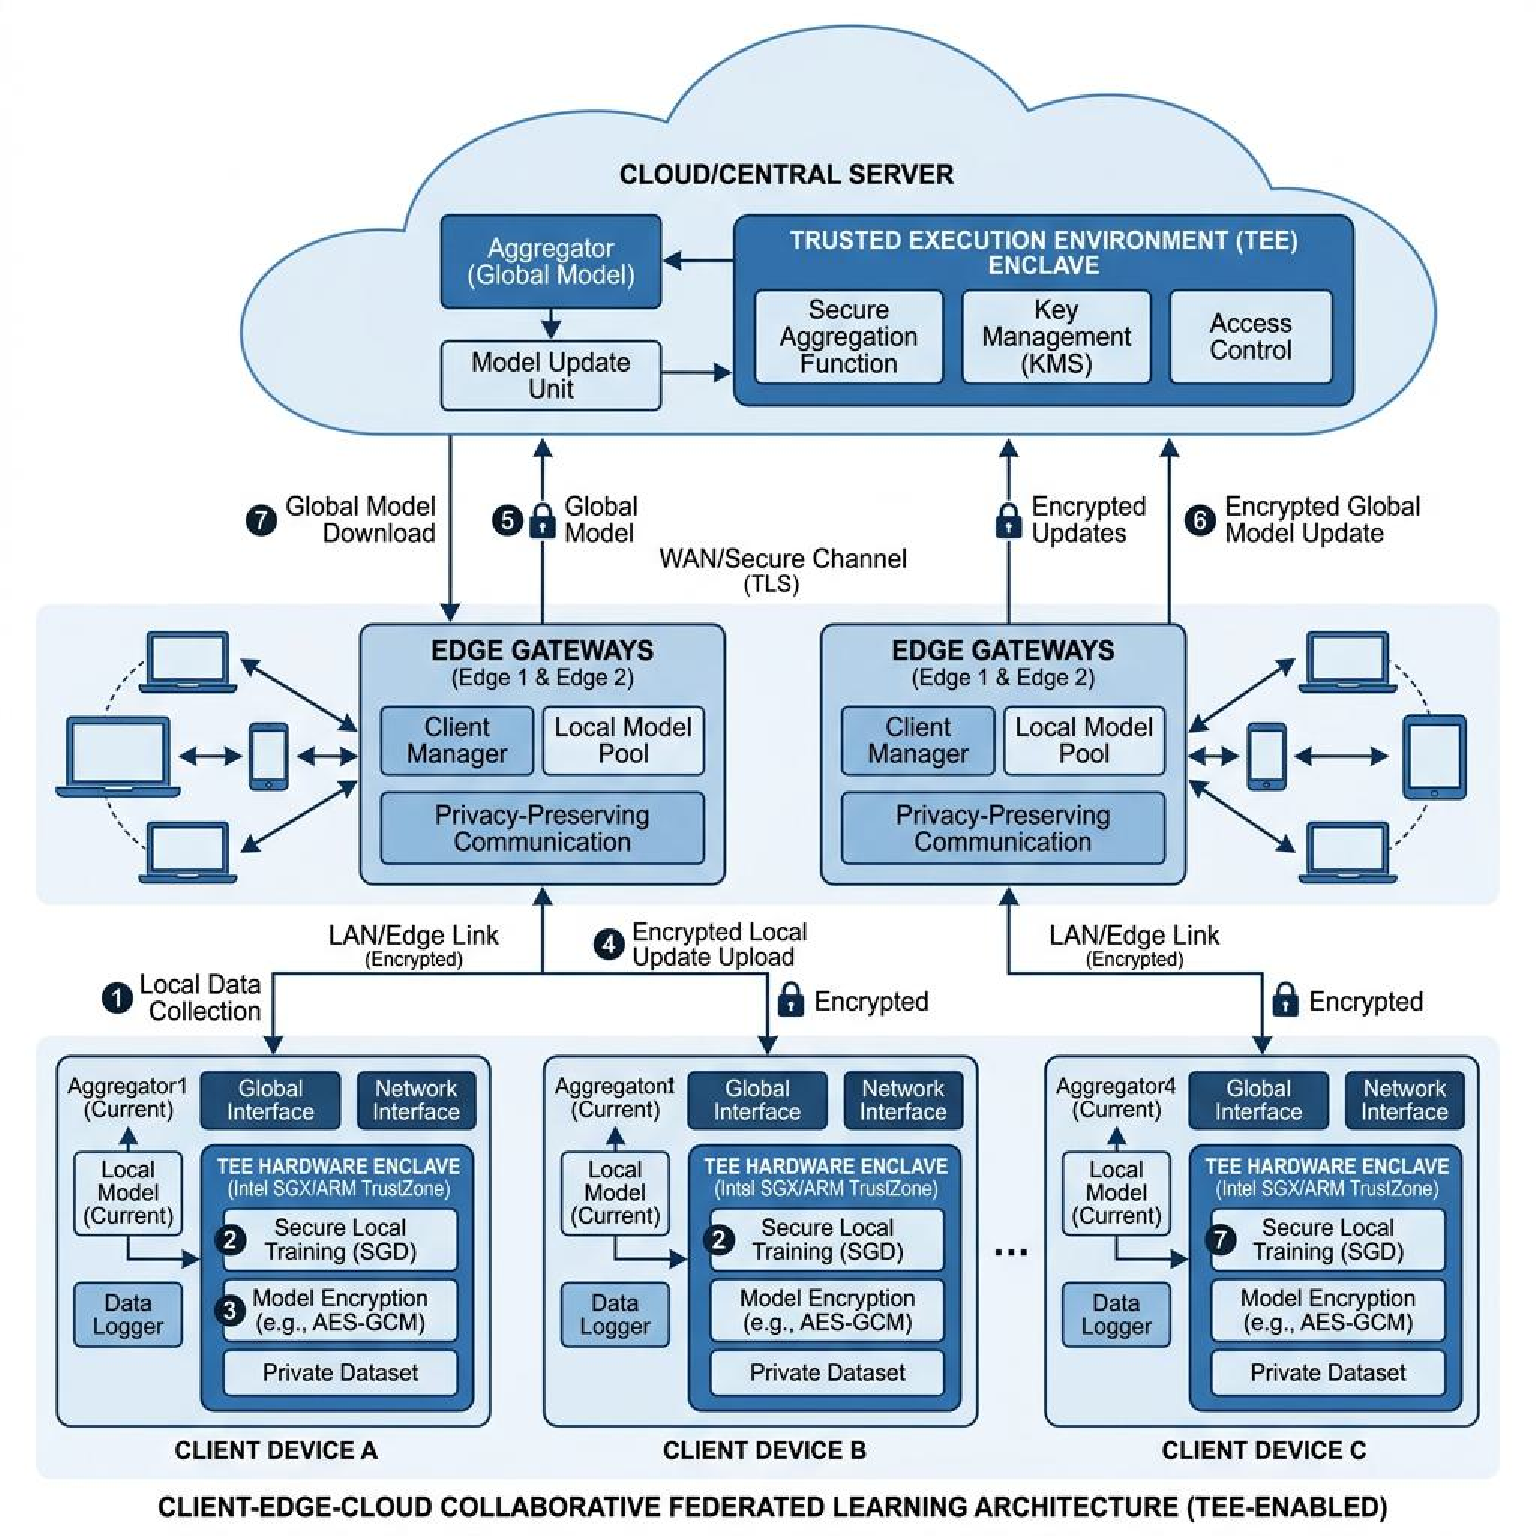
\includegraphics[width=0.85\textwidth]{system_arch.pdf}
    \caption{Client-Edge-Cloud collaborative architecture with TEE-anchored trust verification.}
    \label{fig:system_arch}
\end{figure}

The system initially establishes TEE encrypted channels within the kernel of each edge device $c_k$ by deploying hard access credentials, and subsequently executes its joint modeling objective: minimizing the expected empirical risk over the aggregate data distributions $\mathcal{D}_k$ across all physical edge entities:
\begin{equation}
\min_{W} \mathcal{L}(W) = \sum_{k=1}^K p_k \mathcal{L}_k(W)
\end{equation}
where $p_k = |\mathcal{D}_k| / \sum |\mathcal{D}_j|$. At the dawn of the $t$-th training round, the server broadcasts a baseline model replica $W_{global}^{(t-1)}$. The secure agent nodes (starting from $W_{k,0}^{(t)} \equiv W_{global}^{(t-1)}$) perform $E$ rounds of local Stochastic Gradient Descent (SGD) computations using a localized learning rate $\eta_l$ over their Non-IID datasets. The resulting localized parameter increment can be expressed as an accumulative tensor shift:
\begin{equation}
\Delta W_{k}^{(t)} = W_{k, E}^{(t)} - W_{global}^{(t-1)}, \quad \text{where } W_{k, e}^{(t)} = W_{k, e-1}^{(t)} - \eta_l \nabla \mathbb{E}[\ell(W_{k, e-1}^{(t)}; x, y)]
\end{equation}
where the expectation $\mathbb{E}[\cdot]$ denotes the mathematical expectation sampled via randomized mini-batches over the local dataset $\mathcal{D}_k$ (the batch size is uniformly set to 64 in the simulation framework configuration of this study).

Finally, legitimate increments along with their TEE-signed attestation quotes are uploaded to the server, which implements robust updates via a multi-stream trust-scoring system:
\begin{equation}
W_{global}^{(t)} = W_{global}^{(t-1)} + \mathrm{Agg}(\{ \Delta W_{k}^{(t)} \}_{k\in\Phi})
\end{equation}
where $\Phi \subseteq \mathcal{C}$ denotes the set of clients surviving trust-based filtering in the current round, and $\mathrm{Agg}(\cdot)$ represents the secure aggregation operator detailed in Section~4.


\subsection{Threat Model}
A sound security framework must clearly delineate the adversarial capabilities and trust assumptions. This section specifies three tiers of entities and the corresponding trust boundaries (the multi-dimensional attack surfaces are illustrated in Fig.~\ref{fig:threat_model}):
\begin{itemize}
    \item \textbf{Hardware Isolation Assumption (Trust Anchor)}:
    Under standard cryptographic assumptions---excluding physical side-channels and microarchitectural timing attacks~\cite{zhang2025rppfl}---we assume that even if the host OS is fully compromised, the TEE enclave (e.g., TrustZone, SGX) maintains its isolation guarantees.
    This provides a tamper-resistant root for unforgeable attestation reports.
    \item \textbf{Honest-but-Curious Aggregation Server}: The central server faithfully executes the prescribed aggregation protocol without deviation, but may attempt to infer private information from the received model updates.
    \item \textbf{Internal Colluding Adversaries}: Unlike external passive eavesdroppers, we assume adversaries have compromised a fraction of legitimate devices (upper bound $< 50\%$). These malicious insiders can arbitrarily tamper with local labels, inject poisoned samples (including clean-label attacks), or directly manipulate gradient tensors (e.g., sign-flipping or magnitude scaling). Although the theoretical tolerance extends to 50\%, our primary benchmarks operate at the high-intensity 30\% setting; the 50\% extreme scenario serves as an independent stress test of system resilience.
\end{itemize}

\begin{figure}[htbp!]
    \centering
    
\includegraphics[width=0.75\textwidth]{threat_model.pdf}
    \caption{Multi-dimensional composite poisoning threat model in edge federated networks.}
    \label{fig:threat_model}
\end{figure}

\subsection{Design Goals}
Under the above threat model with 30--50\% malicious participation and severe data heterogeneity, this framework targets three objectives:
\begin{enumerate}
    \item \textbf{High True-Positive Detection with Stable Convergence}: The system must reliably identify and exclude all malicious participants regardless of their camouflage strategies, achieving near-100\% true-positive recall while suppressing the backdoor ASR to a minimal level and maintaining robust global model convergence.
    \item \textbf{Zero False-Positive Tolerance for Heterogeneous Clients}: Unlike rigid threshold-based defenses that frequently misclassify legitimate long-tail nodes, the framework allows compliant clients with skewed data distributions to recover participation rights via temporal reputation accumulation, driving the long-term FPR toward zero.
    \item \textbf{Low Computational and Communication Overhead}: Avoiding heavyweight cryptographic primitives such as Fully Homomorphic Encryption or Zero-Knowledge Proofs, the system concentrates its overhead on lightweight hardware attestation and orthogonal trust state tracking, ensuring compatibility with resource-constrained edge devices (e.g., LXC/Docker containers).
\end{enumerate}

\section{Proposed Method: Trust Flow-Driven Trusted Federated Framework}

This section presents the proposed \emph{Trust Flow-Driven Trusted Federated Learning} defense architecture. The core idea is to decompose each federated round into five synergistic phases: (1)~hardware-anchored admission, (2)~reference-based content auditing, (3)~orthogonal state evolution, (4)~layer-wise risk-gated aggregation, and (5)~global update dispatch. Rather than relying on isolated point defenses, the framework propagates and tracks holistic \textbf{Trust Flows} across all five phases, forming a persistent closed-loop regulatory mechanism.

For clarity of subsequent formulations, Table~\ref{tab:notations} summarizes the key notations used throughout this paper.

\begin{table}[htbp]
\centering
\caption{Core System Parameters and Trust Flow Symbolic Notations.}
\label{tab:notations}
\resizebox{\textwidth}{!}{
\begin{tabular}{cl | cl}
\toprule
\textbf{Symbol} & \textbf{Description} & \textbf{Symbol} & \textbf{Description} \\
\midrule
$W_{global}^{(t)}$ & Global model parameters at round $t$ & $\mathcal{A}$ & Set of active nodes admitted to aggregation \\
$\Delta W_k$ & Local model update from client $k$ & $\Phi^{(l)}$ & Set of survivors admitted at layer $l$ \\
$TrustScore_k$ & TEE-anchored initial trust score & $HistPerf_k$ & Historical performance accumulator ($\in [0, 1]$)\\
$ContentScore_k$ & Current-round content quality score & $RiskEMA_k$ & Instantaneous risk indicator ($\in [0, 1]$)\\
$RawScore_k$ & Fused multi-dimensional score with risk discount & $M_{attest,k}$ & Hardware remote attestation pass flag \\
$g_{root}$ & Server-side clean reference gradient & $A_k$ & Runtime anomaly metric for client $k$ \\
\bottomrule
\end{tabular}
}
\end{table}

\begin{figure}[htbp]
    \centering
    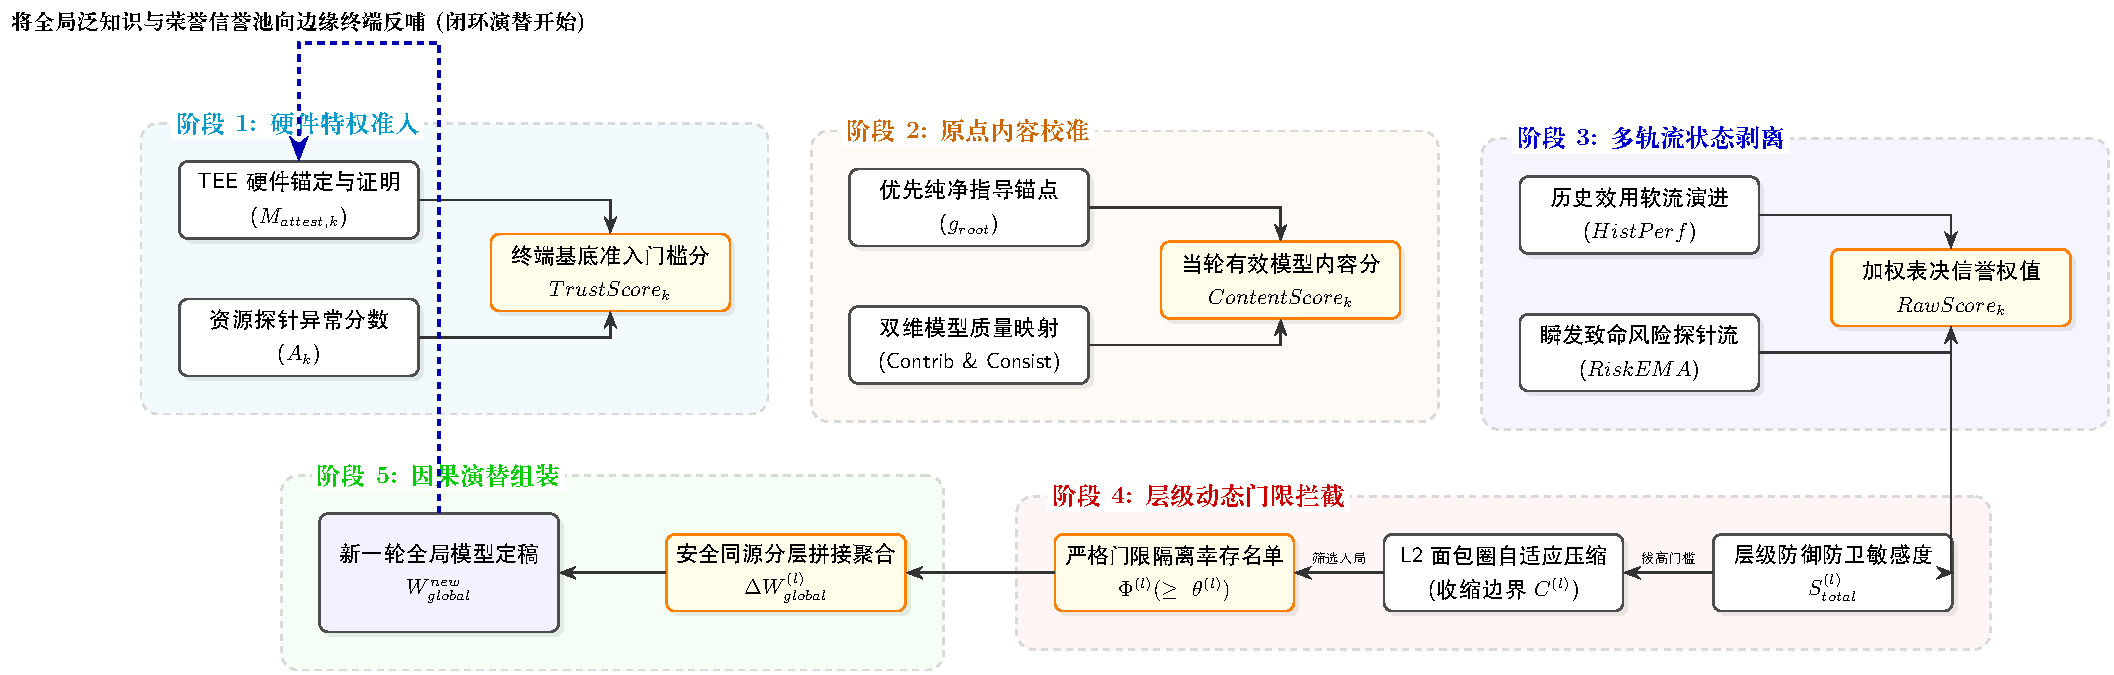
\includegraphics[width=\textwidth]{fig3_arch.pdf}
    \caption{Holistic Architectural Outline of the Trust Flow-Driven Five-stage Closed-Loop Defense.}
    \label{fig:framework}
\end{figure}

\subsection{Phase 1: Hardware-Anchored Client Admission and Initial Trust Scoring}
To proactively block Sybil nodes with forged identities and compromised devices running in breached environments, the system deploys a \textbf{Trusted Management Attestation Agent (TMAA)} based on Trusted Execution Environments (TEE).
Before each training round, every client must submit a Remote Attestation Quote---containing Platform Configuration Register (PCR) measurements---generated from non-exportable Hardware Device Unique Keys (DUKs). A client passing attestation verification receives $M_{attest,k} = 1$; otherwise $M_{attest,k} = 0$ and the client is immediately rejected.

For admitted nodes, the server derives a behavioral anomaly metric $A_k \in [0, \infty)$ from TMAA-monitored runtime indicators (e.g., CPU utilization patterns and process integrity checks). The initial trust score $TrustScore_k \in [0, 1]$ is then computed as:
\begin{equation}
    TrustScore_{k} = M_{attest,k} \cdot \exp\left(-\lambda \cdot\max(0, A_{k} - \tau)^{\rho}\right),
\end{equation}
where $\lambda$ controls the penalty steepness for anomaly deviations, $\tau$ defines a tolerance dead-zone for normal operational variance, and $\rho$ governs the decay acceleration. Default values are $\lambda=5.0$, $\tau=0.1$, $\rho=2.0$ (see Section~\ref{sec:experiments} for the full parameter matrix).

\subsection{Phase 2: Server-Prioritized Reference Construction and Content Auditing}
Computing cosine similarity directly between client gradients is vulnerable to coordinated collusion attacks. To mitigate this, the framework constructs a trusted \textbf{server-side reference direction}.
If the server maintains a small clean validation set, it computes the reference gradient $g_{root\_clean}$ directly on the current global model. Otherwise, the reference is constructed as a trust-weighted combination of client updates, where weights incorporate both the hardware trust score and the previous round's risk assessment:
\begin{equation}
    \omega_{k}^{ref} = TrustScore_{k} \cdot (1 - RiskEMA_{k}^{prev})^{2}.
\end{equation}
The unified reference gradient for round $t$ is thus:
\begin{equation}
    g_{root}=
    \begin{cases}
        g_{root\_clean}, & \text{if clean server data is available}, \\
        \sum_{k} \frac{\omega_{k}^{ref}}{\sum_j \omega_{j}^{ref}} \Delta W_k, & \text{otherwise}.
    \end{cases}
\end{equation}

Given $g_{root}$, the server evaluates each client's \emph{Content Quality Score} by fusing two complementary metrics: (i)~\emph{Contribution Alignment}, measuring the cosine similarity between $\Delta W_k$ and $g_{root}$, and (ii)~\emph{Group Consistency}, measuring agreement with the trusted majority. These are combined via a weighted harmonic mean:
\begin{align}
    S_{contrib,k} &= \max\left(0,\ \alpha_{1} + \alpha_{2} \cdot \cos(\Delta W_{k}, g_{root})\right), \\
    S_{consist,k} &= \frac{\sum_{j\neq k} TrustScore_{j} \cdot \max\left(0,\ \alpha_{1} + \alpha_{2} \cdot \cos(\Delta W_{k}, \Delta W_{j})\right)}{\sum_{j\neq k} TrustScore_{j} + \varepsilon}, \\
    ContentScore_{k} &= \frac{(1 + \beta_{fusion}^{2}) \cdot S_{consist,k} \cdot S_{contrib,k}}{\beta_{fusion}^{2}\cdot S_{consist,k} + S_{contrib,k} + \varepsilon}.
\end{align}
Here, $\alpha_{1}$ and $\alpha_{2}$ ($\alpha_1 + \alpha_2 = 1.0$) calibrate the cosine mapping range, while $\beta_{fusion} > 1.0$ (empirically set to 2.0) biases the fusion toward contribution alignment over group consistency. This prioritization of the clean reference strengthens resilience against coordinated collusion.

\begin{algorithm}[htbp]
\caption{Admissions and Content Auditing Grounded on Hardware Anchors and Pristine References}
\label{alg:phase12}
\begin{algorithmic}[1]
\REQUIRE Client set $\mathcal{C}$, local updates $\{\Delta W_k\}_{k\in\mathcal{C}}$, previous risk states $RiskEMA^{(t-1)}$
\ENSURE $TrustScore_k$, $ContentScore_k$, reference gradient $g_{root}$
\STATE \textbf{Stage 1: Hardware Attestation}
\FOR{each client $k \in \mathcal{C}$}
    \IF{$M_{attest,k} == 1$ (TEE attestation passed)}
        \STATE Obtain runtime anomaly metric $A_k$
        \STATE $TrustScore_k \leftarrow \exp(-\lambda \max(0, A_k-\tau)^\rho)$
    \ELSE
        \STATE Reject client: $TrustScore_k \leftarrow 0$
    \ENDIF
\ENDFOR
\STATE \textbf{Stage 2: Reference Construction and Content Auditing}
\IF{Server holds clean validation data}
    \STATE Compute clean reference: $g_{root} \leftarrow g_{root\_clean}$
\ELSE
    \STATE Compute trust-weighted coefficients $\omega_k^{ref} \leftarrow TrustScore_k \cdot (1 - RiskEMA_k^{(t-1)})^2$
    \STATE Aggregate reference: $g_{root} \leftarrow \sum_k (\omega_k^{ref} \Delta W_k) / \sum_j \omega_j^{ref}$
\ENDIF
\FOR{each admitted client $k$}
    \STATE Contribution alignment $S_{contrib,k} \leftarrow \max(0, \alpha_1 + \alpha_2 \cos(\Delta W_k, g_{root}))$
    \STATE Group consistency $S_{consist,k} \leftarrow \frac{\sum_{j \neq k} TrustScore_j \max(0, \alpha_1 + \alpha_2 \cos(\Delta W_k, \Delta W_j))}{\sum_{j \neq k} TrustScore_j + \varepsilon}$
    \STATE Fused content score $ContentScore_k \leftarrow \frac{(1+\beta_{fusion}^2)S_{consist,k} S_{contrib,k}}{\beta_{fusion}^2 S_{consist,k} + S_{contrib,k} + \varepsilon}$
\ENDFOR
\RETURN $\{TrustScore_k, ContentScore_k, g_{root}\}$
\end{algorithmic}
\end{algorithm}

\subsection{Phase 3: Orthogonal State Evolution of Historical Performance Flow and Instant Risk Flow}
Traditional single-metric reputation mechanisms inherently struggle against heterogeneous data limitations. The intrinsic defense pivot adopted mathematically inside this framework leverages absolute "dimensional decoupling", disassembling chronological measurements into twin opposing and firmly distinct temporal progression tracks: deploying the \textbf{Historical Performance Flow ($HistPerf$)} to manage resilient permission allowances, structurally distanced from the definitive penalization veto governed strictly by the \textbf{Instantaneous Risk Containment Flow ($RiskEMA$)}.

\textbf{(1) Historical Performance Flow ($HistPerf$)} primarily undertakes the evaluation of long-term capabilities. It does not possess the authority to make "negative decisions". In each round, based on the relative standard deviation distribution (the $z$-score) of the $ContentScore$ across the entire queue, a smoothing function and a baseline threshold are weighted to derive the increment $Signal_k^{upd}$:
\begin{align}
    z_{k} &= \frac{ContentScore_{k} - \mu_{content}}{\sigma_{content} + \varepsilon}, \quad Signal_{k}^{rel} = \sigma(z_{k}), \\
    Signal_{k}^{abs} &= \mathrm{clip}\left(\frac{ContentScore_{k} - b}{s}, 0, 1\right), \\
    Signal_{k}^{upd} &= \gamma_{rel} \cdot Signal_{k}^{rel} + \gamma_{abs} \cdot Signal_{k}^{abs}, \\
    HistPerf_{k}^{(t)} &= \beta_{h} \cdot HistPerf_{k}^{(t-1)} + (1 - \beta_{h}) \cdot Signal_{k}^{upd}.
\end{align}
Here, the constants $b$ and $s$ serve as scaling boundaries for the absolute score; $\gamma_{rel}$ and $\gamma_{abs}$ (which sum to $1.0$) adjust the proportions of relative competition and absolute performance, respectively. When $HistPerf$ is extremely low, the node is simply placed into a temporary seat termed "Hist Soft Isolation" (unable to participate in the current round's aggregation, but remaining within the network). This design preserves unpopular data nodes.

\textbf{(2) Instantaneous Risk Containment Flow ($RiskEMA$)} is the core mechanism for intercepting attackers. It bypasses simple gradient angle matching and comprehensively adopts multi-dimensional probe data from gradients (loss oscillation $r_{probe}$, neuronal polarity distribution $r_{grad}$, stealth backdoor channels $r_{trigger}$, and even image-level pre-screening $r_{pixel}$). We extract the highest instantaneous extremum across all risk probe channels in each round:
\begin{equation}
    Risk_{k}^{inst} = \max\{r_{report}, r_{grad}, r_{probe}, r_{pixel}, r_{trigger}, r_{sign}, r_{peer}, \dots \},
\end{equation}
Subsequently, exponential decay memory is applied backward (with $\beta_r = 0.85$ acting as the smoothing coefficient):
\begin{equation}
    RiskEMA_{k}^{(t)} = \beta_{r} \cdot RiskEMA_{k}^{(t-1)} + (1 - \beta_{r}) \cdot Risk_{k}^{inst}.
\end{equation}

By combining the orthogonal calculus of the aforementioned multi-dimensional risks and historical utilities, the framework establishes a secure lifecycle state transition automaton for all nodes within the controlled federation (its topology is illustrated in Fig.~\ref{fig:node_state_machine}), delineating four major supervision quadrants:
\begin{itemize}
    \item \textbf{Normal Nodes (NORMAL)}: Fully participate in the current round's aggregation and distribution. When the probe acutely captures an anomaly (a rise in RiskEMA) or a decline in historical utility, the node will shift rightwards to the suspect status or transition into the soft isolation state, respectively.
    \item \textbf{Suspect Nodes (SUSPECT)}: Localized monitoring is intensified on the dimension that triggered the alarm. If the observed risk subsides, it is pardoned and restored to NORMAL; if it continuously triggers the redline threshold, it is handed over to the isolation procedure.
    \item \textbf{Quarantine Observation (QUARANTINE)}: The node is excluded from contributing parameters to the current global aggregation, retaining only non-critical computation rights. If subsequent observations confirm compliance, it may return to NORMAL; otherwise, persistent violations trigger permanent banning.
    \item \textbf{Blacklist Banning (BLACKLIST)}: A permanent, irreversible blacklist. Hitting the hard threshold completely severs the handshake at the TEE certificate layer, terminating all future collaborative qualifications.
\end{itemize}
This state decoupling mechanism, which balances historical tolerance with immediate risk response, enables the framework to aggressively filter suspicious gradients while maintaining a false positive rate converging to zero.

\begin{figure}[htbp]
    \centering
    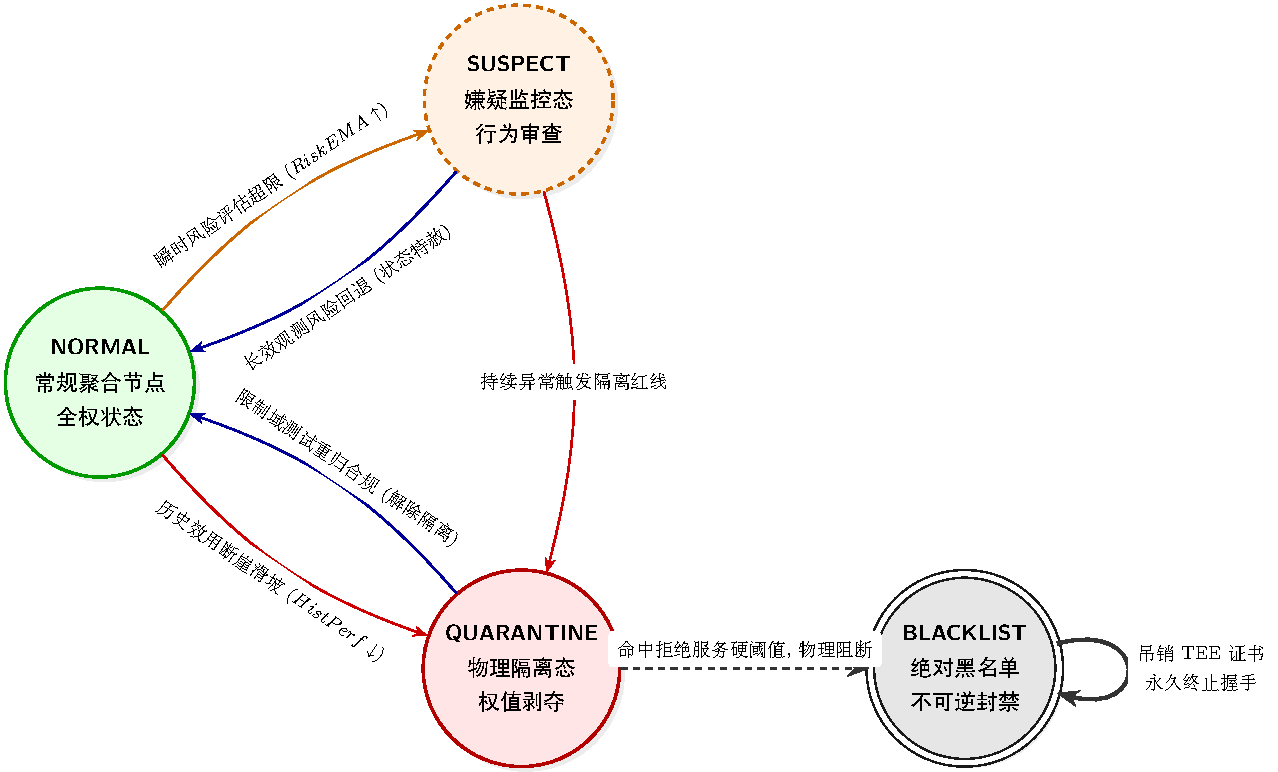
\includegraphics[width=0.9\textwidth]{fig4_state.pdf}
    \caption{Logical diagram of the four-state supervision transition automaton under the superposition of client historical accumulation and instantaneous risks.}
    \label{fig:node_state_machine}
\end{figure}

Finally, $TrustScore$ (hardware reputation), $ContentScore$ (effort in the current round), and $HistPerf$ (historical prestige) converge into a base metric for the absolute weight of the current round's aggregation, yielding $RawScore_k$ after applying a risk discount:
\begin{align}
    RawScore_{k}^{base} &= (TrustScore_{k})^{\alpha} \cdot (ContentScore_{k})^{\beta} \cdot (HistPerf_{k}^{(t-1)})^{\gamma}, \\
    RawScore_{k} &= RawScore_{k}^{base} \cdot (1 - RiskEMA_{k}^{prev})^{p},
\end{align}
where the exponential hyperparameters $\alpha, \beta, \gamma$, and $p$ sequentially determine the control strength of the four aforementioned dimensions over the final voice (weight feedback).

\begin{algorithm}[htbp]
\caption{Dual-stream Orthogonal Trust State Evolution (HistPerf \& RiskEMA)}
\label{alg:phase3}
\begin{algorithmic}[1]
\REQUIRE $ContentScore_k$, Multi-dimensional risk probe set $\{r_{probe}, r_{grad}, \dots\}$
\ENSURE $HistPerf_k^{(t)}$, Instantaneous risk flow $RiskEMA_k^{(t)}$, Global weight baseline score $RawScore_k$
\STATE \textbf{Stream A: Historical Utility Flow Evolution (Competitive Soft Privilege)}
\STATE Calculate the global mean $\mu_{content}$ and standard deviation $\sigma_{content}$ of the content scores
\FOR{each admitted client $k$}
    \STATE Relative competition signal $Signal_k^{rel} \leftarrow \sigma((ContentScore_k - \mu_{content})/(\sigma_{content} + \varepsilon))$
    \STATE Absolute baseline signal $Signal_k^{abs} \leftarrow \mathrm{clip}((ContentScore_k - b)/s, 0, 1)$
    \STATE Comprehensive increment $Signal_k^{upd} \leftarrow \gamma_{rel} Signal_k^{rel} + \gamma_{abs} Signal_k^{abs}$
    \STATE Update $HistPerf_k^{(t)} \leftarrow \beta_h HistPerf_k^{(t-1)} + (1 - \beta_h) Signal_k^{upd}$
\ENDFOR
\STATE \textbf{Stream B: Instantaneous Risk Disciplinary Flow Evolution (One-vote Veto Power)}
\FOR{each client $k$}
    \STATE Capture the instantaneous risk extremum $Risk_k^{inst} \leftarrow \max\{r_{report}, r_{grad}, r_{probe}, r_{pixel}, r_{trigger}\}$
    \STATE Update $RiskEMA_k^{(t)} \leftarrow \beta_r RiskEMA_k^{(t-1)} + (1-\beta_r) Risk_k^{inst}$
    \IF{$RiskEMA_k^{(t)} > \text{Isolation Threshold}$}
        \STATE Add to long-term isolation blacklist $RiskIsolated \leftarrow RiskIsolated \cup \{k\}$
    \ENDIF
\ENDFOR
\STATE \textbf{Final Privilege Fusion Calculation}
\FOR{each active client $k \notin RiskIsolated$}
    \STATE Fusion score $RawScore_k \leftarrow (TrustScore_k)^\alpha (ContentScore_k)^\beta (HistPerf_k^{(t-1)})^\gamma$
    \STATE Risk discount $RawScore_k \leftarrow RawScore_k \cdot (1 - RiskEMA_k^{(t-1)})^p$
\ENDFOR
\RETURN $\{HistPerf_k^{(t)}, RiskEMA_k^{(t)}, RawScore_k\}$
\end{algorithmic}
\end{algorithm}

\subsection{Phase 4: Risk-gated Layer-wise Differentiated Robust Aggregation}
The attacker's stealthy backdoors are frequently concealed inside specific neurons within deep layers. A naive full-model aggregation that uniformly merges all gradient components leaves vulnerabilities for dormant backdoors to penetrate. Therefore, we propose a differentiated (Layer-wise) admission-gated aggregation strategy executed according to the network layer depth $l$.

First, filter the set of active clients $\mathcal{A}$ qualified to participate in the current round:
\begin{equation} \label{eq:active_clients}
    \mathcal{A} = \{k \mid k \notin RiskIsolated \land k \notin HistSoftIsolated\}.
\end{equation}

Second, for the $l$-th layer, evaluate its security defense requirements. Shallow layers typically preserve common low-level features such as edges and textures, while deep layers entail massive weight alterations (utility) and are susceptible to buried poison (security). The algorithm leverages a 3D modeling of the weight sensitivity of the layer $S_{total}^{(l)}$:
\begin{align}
    S_{privacy}^{(l)} &= \exp\left(-\tau_{p} \frac{l}{L}\right), \\
    S_{utility}^{(l)} &= \frac{\|g_{ref}^{(l)}\|_{2}}{\max_{m}\|g_{ref}^{(m)}\|_{2} + \varepsilon}, \\
    S_{security}^{(l)} &= 1 - \frac{\sum_{k\in\mathcal{A}}TrustScore_{k}\cdot\cos(\Delta W_{k}^{(l)}, g_{ref}^{(l)})}{\sum_{k\in\mathcal{A}}TrustScore_{k} + \varepsilon}, \\
    S_{total}^{(l)} &= w_p S_{privacy}^{(l)} + w_u S_{utility}^{(l)} + w_s S_{security}^{(l)}.
\end{align}
Here, $w_p, w_u, w_s$ denote the hierarchical requirement weighting factors satisfying the normalization condition. When $S_{total}^{(l)}$ is high, the layer is identified as a high-risk target for backdoor injection. The system accordingly elevates the admission threshold $\theta^{(l)} = \mu_{base} + \lambda_{s} \cdot S_{total}^{(l)}$ and tightens the L2 clipping bound $C^{(l)} = C_{base} / (S_{total}^{(l)} + \varepsilon_{c})$.

Third, only those ``layer survivors'' $\Phi^{(l)}$ whose current round $RawScore_k$ exceeds $\theta^{(l)}$ are allowed to submit updates for aggregation. After entering the survivor list, a normalized weight distribution $\tilde{w}_{k}^{(l)}$ is applied and excessively large gradient magnitudes are clipped ($scale_k^{(l)}$):
\begin{align}
    \Phi^{(l)} &= \{k \in \mathcal{A} \mid RawScore_{k} \ge \theta^{(l)} \}, \quad \tilde{w}_{k}^{(l)} = \frac{RawScore_{k}}{\sum_{j\in\Phi^{(l)}}RawScore_{j} + \varepsilon}, \\
    scale_{k}^{(l)} &= \max\left(1, \frac{\|\Delta W_{k}^{(l)}\|_{2}}{C^{(l)}}\right), \quad
    \widehat{\Delta W}_{k}^{(l)} = \frac{\Delta W_{k}^{(l)}}{scale_{k}^{(l)}}.
\end{align}
Fourth, the individual layers are respectively weighted and merged into a single-layer increment:
\begin{equation}
    \Delta W_{global}^{(l)} = \sum_{k\in\Phi^{(l)}}\tilde{w}_{k}^{(l)} \cdot \widehat{\Delta W}_{k}^{(l)},
\end{equation}


\begin{algorithm}[htbp]
\caption{Risk-gated Layer-wise Differentiated Aggregation and Dynamic Clipping}
\label{alg:phase4}
\begin{algorithmic}[1]
\REQUIRE Active nodes $\mathcal{A}$, scores $RawScore_k$, layer-wise update gradients $\{\Delta W_k^{(l)}\}$, network depth $L$
\ENSURE The integrated secure global gradient for the current round $\Delta W_{global}$
\STATE Initialize global increment $\Delta W_{global} \leftarrow 0$
\FOR{each network layer $l = 1, 2, \dots, L$}
    \STATE \textbf{Step 1: 3D Joint Calculation of Layer Sensitivity}
    \STATE Privacy sensitivity $S_{privacy}^{(l)} \leftarrow \exp(-\tau_p \cdot l/L)$
    \STATE Utility sensitivity $S_{utility}^{(l)} \leftarrow \|g_{ref}^{(l)}\|_2 / \max_m\|g_{ref}^{(m)}\|_2$
    \STATE Security sensitivity $S_{security}^{(l)} \leftarrow 1 - \frac{\sum_{k\in\mathcal{A}} TrustScore_k \cos(\Delta W_k^{(l)}, g_{ref}^{(l)})}{\sum_{k\in\mathcal{A}} TrustScore_k + \varepsilon}$
    \STATE Total defense requirement sensitivity $S_{total}^{(l)} \leftarrow w_p S_{privacy}^{(l)} + w_u S_{utility}^{(l)} + w_s S_{security}^{(l)}$
    \STATE \textbf{Step 2: Dynamic Risk Gating and Adaptive L2 Norm Clipping}
    \STATE Elevate the security admission score threshold for this layer $\theta^{(l)} \leftarrow \mu_{base} + \lambda_s \cdot S_{total}^{(l)}$
    \STATE Tighten the malicious amplitude clipping boundary for this layer $C^{(l)} \leftarrow C_{base} / (S_{total}^{(l)} + \varepsilon_c)$
    \STATE \textbf{Step 3: Survivor Node Selection and Secondary Re-calibration}
    \STATE Filter the survivor list for this layer $\Phi^{(l)} \leftarrow \{k \in \mathcal{A} \mid RawScore_k \ge \theta^{(l)}\}$
    \STATE Re-normalize the effective weights for the survivors $\tilde{w}_k^{(l)} \leftarrow RawScore_k / \sum_{j\in\Phi^{(l)}} RawScore_j$
    \STATE Execute L2 proportional downscaling $\widehat{\Delta W}_k^{(l)} \leftarrow \Delta W_k^{(l)} / \max(1, \|\Delta W_k^{(l)}\|_2 / C^{(l)})$
    \STATE \textbf{Step 4: Layer-wise Merging and Stitching}
    \STATE Aggregate filtered gradients for this layer $\Delta W_{global}^{(l)} \leftarrow \sum_{k\in\Phi^{(l)}} \tilde{w}_k^{(l)} \cdot \widehat{\Delta W}_k^{(l)}$
    \STATE Splice and integrate into the global model update amount $\Delta W_{global} \leftarrow \Delta W_{global} \cup \Delta W_{global}^{(l)}$
\ENDFOR
\RETURN $\Delta W_{global}$
\end{algorithmic}
\end{algorithm}

\subsection{Phase 5: Global Update Dispatch and Edge Knowledge Retention}
After completing the layer-wise aggregation, the system enters the final closed-loop phase. The server applies the stitched secure increments to the global model: $W_{global}^{new} = W_{global}^{old} + \Delta W_{global}$. This update, along with the updated $HistPerf$ honors of legitimate clients, is distributed back to the edge population. Through the data integration of these five major phases, the system maintains high convergence while effectively excluding latent malicious updates from the aggregation.

\begin{figure}[htbp]
    \centering
    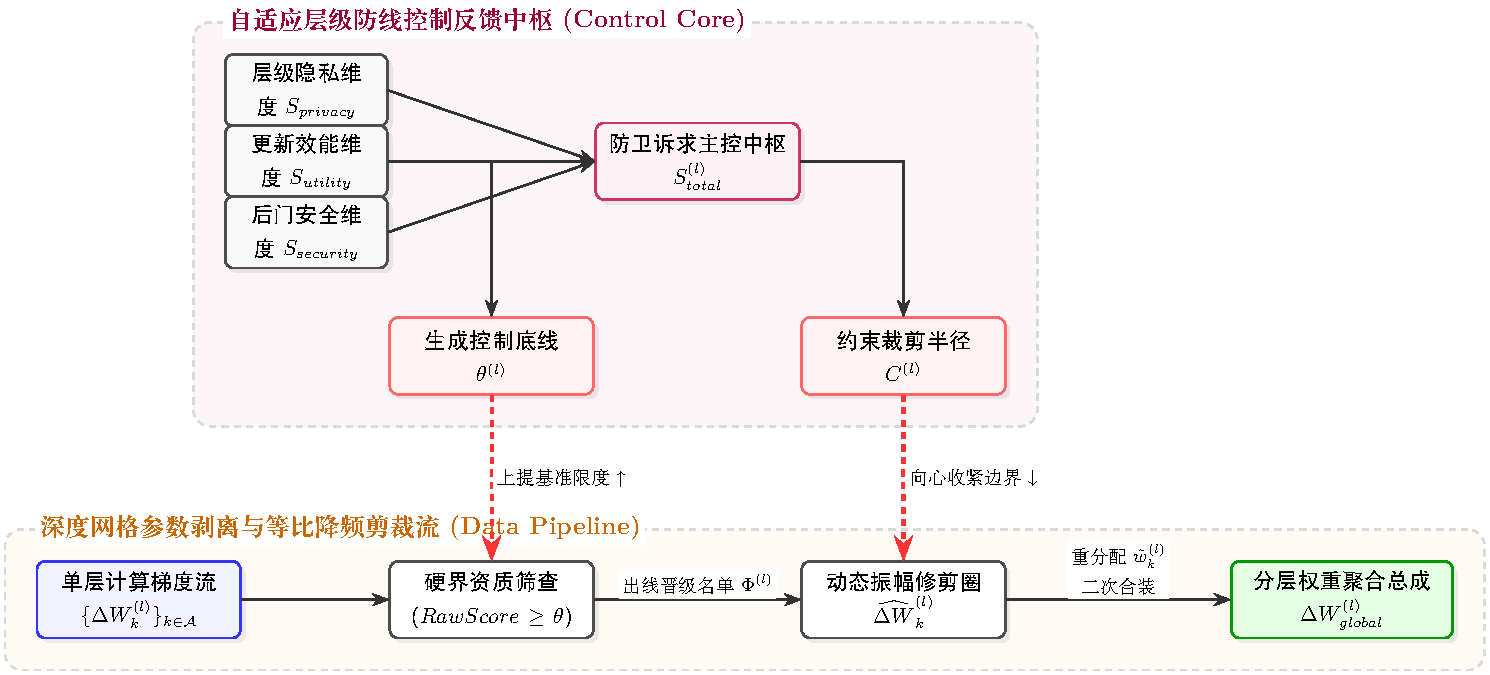
\includegraphics[width=0.95\textwidth]{fig5_layer.pdf}
    \caption{Illustration of risk-gated layer-wise aggregation with adaptive L2 clipping.}
    \label{fig:layer_gating}
\end{figure}

\subsection{Theoretical Guarantee of Dual-stream Orthogonal Decoupling}
Traditional single-domain reputation mechanisms (such as the simple accumulation of cosine similarities) are inherently equivalent to using first-order linear Markov chains to perform one-dimensional projection dimensionality reduction on high-dimensional spaces. In federated environments with strong edge data skewness, this inevitably leads to a trade-off dilemma between False Negatives (FNR) and False Positives (FPR). This section mathematically formalizes how the orthogonal dual-stream framework presented in this paper resolves this mathematical contradiction.

\begin{lemma}[Variance Convergence Properties of Long-tail Nodes]
Assume that the raw content score $ContentScore_{k}^{(t)}$ of a compliant long-tail client $k$ in a single round follows a perturbation distribution with an expectation of $\mu_{clean}$ and an extremely large variance $\sigma_{clean}^2$ caused by Non-IID data. Under a traditional rigid single-line truncation threshold $\tau_{hard}$, when $\tau_{hard} > \mu_{clean} - \sigma_{clean}$, this node faces a high probability of continuous elimination. However, under the historical utility flow smoothing integration rule proposed in this paper, the long-term state expectation of this node is $\mathbb{E}[HistPerf_k^{(\infty)}] = \mu_{clean}$, and the long-term variance is compressed to the limit:
\begin{equation}
    \operatorname{Var}(HistPerf_{k}^{(\infty)}) = \frac{1-\beta_h}{1+\beta_h} \sigma_{clean}^{2}
\end{equation}
Since $0 < \beta_h < 1$, when the tolerance factor $\beta_h \to 1$, single-round perturbations are significantly dissipated in the time domain. As long as the client's true contribution expectation $\mu_{clean}$ is higher than the absolute minimum survival baseline of the system, the integration flow can act as a low-pass filter to guarantee, with probability $P \to 1$, that it survives through instantaneous low score troughs. Consequently, the theoretical False Positive Rate (FPR) approaches zero ($\lim_{t \to \infty} \text{FPR} = 0$).
\end{lemma}

\begin{lemma}[Transient Impulse Response against Advanced Latent Attacks]
Consider a high-level backdoor poisoning node $m$ that adopts a strategy of ``high-frequency camouflage in early stages, extremely rare stealth explosions''. Although its accumulated dividends in early rounds satisfy $\mathbb{E}[HistPerf_m] \ge \mu_{clean}$, when it releases malicious fine-tuning parameters in round $t$, its deep and shallow triggering probe values are significantly higher than the norm (i.e., $\exists r \in \{r_{grad}, r_{probe}, r_{trigger}\}, r \gg 1$). For theoretical analysis, we consider the following lower-bound formulation: since $Risk_k^{inst} = \max\{r_{grad}, r_{probe}, r_{trigger}, \dots\}$, the RiskEMA trajectory is bounded below by the idealized maximum operator:
\begin{equation}
    RiskEMA_m^{(t)} \ge \max \left( \beta_r \cdot RiskEMA_m^{(t-1)},\ \mathcal{F}_{probe}(r_{grad}, r_{probe}, r_{trigger}) \right)
\end{equation}
Because $\mathcal{F}_{probe}$ generates an instantaneous mutation when it detects poisoning features, this causes the risk derivative to exhibit an impulse response approaching the blocking threshold the moment it is triggered, resulting in an immediate categorical isolation.
\end{lemma}

\begin{theorem}[Orthogonal Decoupling of Dual-Stream Blockade]
In the dual-track evaluation mechanism established in this paper, the local Non-IID variance of honest long-tail nodes is smoothed to the low-pass limit in the $HistPerf$ plane. In contrast, any out-of-bounds malicious poisoning gradient will inevitably produce a unilateral jump across the gating blockade threshold due to the lower-bound maximum constraint dictated by the instantaneous $Risk^{inst}$ probes. The system implements an absolute orthogonal analytical isolation for these two types of events with diametrically opposite feature distributions. This theoretically resolves the dimensionality curse of single-score defense lines, which intrinsically fail to balance $\text{FPR} \to 0$ and $\text{ASR} \to 0$ simultaneously.
\end{theorem}

\section{Experiments and Analysis}
\label{sec:experiments}
\subsection{Experimental Setup and Reproducible Parameters}

\subsubsection{Benchmark Environment and System Hardware/Software Stack}
The complete logic of the evaluation experiments in this section is built from scratch based on the Flower (1.5.0) federated learning framework and the PyTorch deep learning engine. To ensure the authenticity of the experiments and the credibility of the system load, all simulation trials are directly deployed on a commercial high-performance computing server with a physical architecture of Inspur NF5468M6. This server is equipped with dual-socket high-frequency CPUs and is provided with full concurrent computing support by 5 independently allocated NVIDIA A10 (24GB) GPUs. The operating system is Ubuntu 20.04.6 LTS alongside a CUDA 12.8 driver environment.

To achieve strict academic reproducibility, the core mapping logs, code repositories, and startup scripts (Bash) involved in the experimental framework are all retained for verification. It is essential to note that to graph a coherent node state tracking plot with logical evolutionary trajectory (e.g., the subsequent trajectory analysis in Fig. \ref{fig:node_state}), we extracted a representative single full-round run slice bound to a specific seed (e.g., \texttt{seed=42}). In contrast, for rigid indicator quantification of global defense performance (such as the final Acc and ASR numerical tables), the system adopts the stable mean expectation after iterating independently for 5 runs with altered random seeds, thereby guaranteeing statistical objectivity.

\subsubsection{Heterogeneous Dataset Partitioning Methods}
The model utilizes a classic lightweight Convolutional Neural Network (CNN) architecture, and the dataset employs the benchmark CIFAR-10. To construct a highly Non-Independent and Identically Distributed (Non-IID) scenario, all 50,000 training images are partitioned and distributed across three categories of groups:
\begin{itemize}
    \item \textbf{Shared Base Pool}: A balanced sample of 5,000 images is extracted and shared among all legitimate nodes to serve as initial knowledge.
    \item \textbf{Weakly Heterogeneous Client Group (Group A, Nodes 6-11)}: Partitioned using a Dirichlet distribution ($\alpha=1.0$), simulating standard edge nodes with slightly skewed but not extremely biased data distributions.
    \item \textbf{Strong Long-tail Heterogeneous Group (Group B \& C, Nodes 12-19)}: Partitioned via a Dirichlet distribution ($\alpha=0.1$); these clients exhibit extremely strong ``partiality'', usually holding massive amounts of data for only a few specific categories. They are highly susceptible to being mistakenly killed by traditional cosine defenses.
\end{itemize}

\subsubsection{Malicious Attack Instances and Proportions}
To examine the comprehensive detection capability of our ``Trust Flow'' defense model, 6 persistently active malicious nodes were mixed into the 20-node network (a high-risk proportion of 30\%). We not only configured traditional data poisoning but also introduced more destructive direct model parameter manipulation attacks:
\begin{itemize}
    \item \textbf{Client 0 - Label Flip Poisoning ($\gamma=0.5$)}: Forcibly maps a certain category in its local real dataset to another category, instilling erroneous boundaries into the network.
    \item \textbf{Client 1 - Stealthy Backdoor Injection ($\gamma=0.2$)}: Applies a specific pixel patch (Trigger) to the corners of 20\% of the training sample images and tags them with the target category 0 label, attempting to mislead the system during inference.
    \item \textbf{Client 2 - Clean Label Backdoor ($\gamma=0.5$)}: This is the most sophisticated attack, utilizing adversarial perturbations to subtly alter the input pixels of target category 0 without modifying its label, thereby confusing gradient feature extraction.
    \item \textbf{Client 3 - Semantic Backdoor Poisoning ($\gamma=0.5$)}: Installs malicious patterns without artificial graphical triggers but directs the model to strongly associate images with specific background colors found in nature entirely with incorrect categories.
    \item \textbf{Client 4 - Sign-Flipping Attack (Model Poisoning)}: The attacker directly manipulates the step-size tensor returned by the underlying PyTorch SGD update, forcibly reversing the signs of gradients in some layers ($\Delta \widehat{W}_k = - \gamma \cdot \Delta W_k$), attempting to trigger severe global convergence deviations and denial of service.
    \item \textbf{Client 5 - Gradient Scaling (Model Poisoning)}: Operating on the basis of a stealthy backdoor, it forcibly magnifies the malicious increment amplitude 100 times ($\Delta \widehat{W}_k = 100 \times \Delta W_k$), attempting to directly overwrite global parameters through a massive weight proportion.
    \item \textbf{Sybil \& Free-rider Nodes}: To empirically validate the efficacy of the Phase 1 TMAA hardware defense line in resisting tampering, the system concurrently initialized 5 Sybil nodes carrying no valid TEE certificates alongside 3 free-rider nodes simulating CPU load dormancy (skipping local epochs to save power) during the initial connection phase.
\end{itemize}

\textbf{Statement on Pre-defense Interception}: All 8 fraudulent nodes (5 Sybil + 3 free-rider) that attempted to join the federation were intercepted at the protocol layer by the TMAA hard gate ($M_{attest,k} = 0$) or disqualified due to anomalous resource utilization signatures detected during the TEE attestation phase. These nodes never participated in any training round.

\begin{table}[htbp]
\centering
\caption{Global Hyperparameters and Defensive Component Optimal Setting Matrix for Physical Platform-based Federated Simulation}
\label{tab:hyperparams}
\resizebox{\textwidth}{!}{
\begin{tabular}{p{4cm} p{7cm} p{3.2cm}}
\toprule
\textbf{Module Architecture Category} & \textbf{Defensive Component Hyperparameter Meaning} & \textbf{Value} \\
\midrule
\multirow{2}{*}{\textbf{Base Config \& Epochs}} & Nodes $K$ & $20$  \\
& Local SGD ($lr$, Momentum) & $0.001$, $0.9$ \\
\midrule
\multirow{3}{*}{\textbf{Phase 1 $\to$ 3 Dual Stream}} & TMAA bound limits $\lambda$, dead-zone $\tau$, factor $\rho$ & $5.0$, $0.1$, $2.0$ \\
& Constraints $\alpha_1, \alpha_2$ and fusion $\beta_{fusion}$ & $0.6$, $0.4$, $2.0$ \\
& History retention $\beta_h$ \& Risk half-life $\beta_r$ & $0.9$, $0.85$ \\
\midrule
\multirow{2}{*}{\textbf{Phase 4 Clipping}} & Score blending non-linear gates ($\alpha, \beta, \gamma, p$) & $3.0, 1.0, 0.5, 1.0$ \\
& Base threshold $\mu_{base}$ and multiplier $\lambda_s$  & $0.4$, $1.2$ \\
\bottomrule
\end{tabular}
}
\end{table}

\subsection{Empirical Analysis of Defense Effectiveness}

\subsubsection{Global Convergence and Attack Prevention Performance}
\textbf{High-Risk Model Boundary (50\% Malicious Ratio) Extended Stress Test}: To thoroughly validate the threat model premise regarding the system's tolerance limit of "high-risk ratio $< 50\%$," we established an extreme confrontation architecture independently (incorporating 10 malicious nodes vs 10 benign ones).

\begin{table}[htbp]
\centering
\caption{\textbf{Comparison of 50\% Limit Stress Test against Standard 30\% Baseline}}
\vspace{4pt}
\label{tab:half_malicious}
\begin{tabular}{l c c c c}
\toprule
\textbf{Experimental Setting} & \textbf{Acc (\%)} & \textbf{ASR (\%)} & \textbf{TPR (\%)} & \textbf{FPR (\%)} \\
\midrule
Standard Baseline (30\% Malicious) & 92.31 $\pm 0.09$ & 10.21 $\pm 0.05$ & 100 & 0.00 \\
\textbf{Extreme Test (50\% Malicious)} & \textbf{91.81 $\pm 0.10$} & \textbf{10.46 $\pm 0.06$} & \textbf{100} & \textbf{0.00} \\
\bottomrule
\end{tabular}
\end{table}

\begin{figure}[htbp]
    \centering
    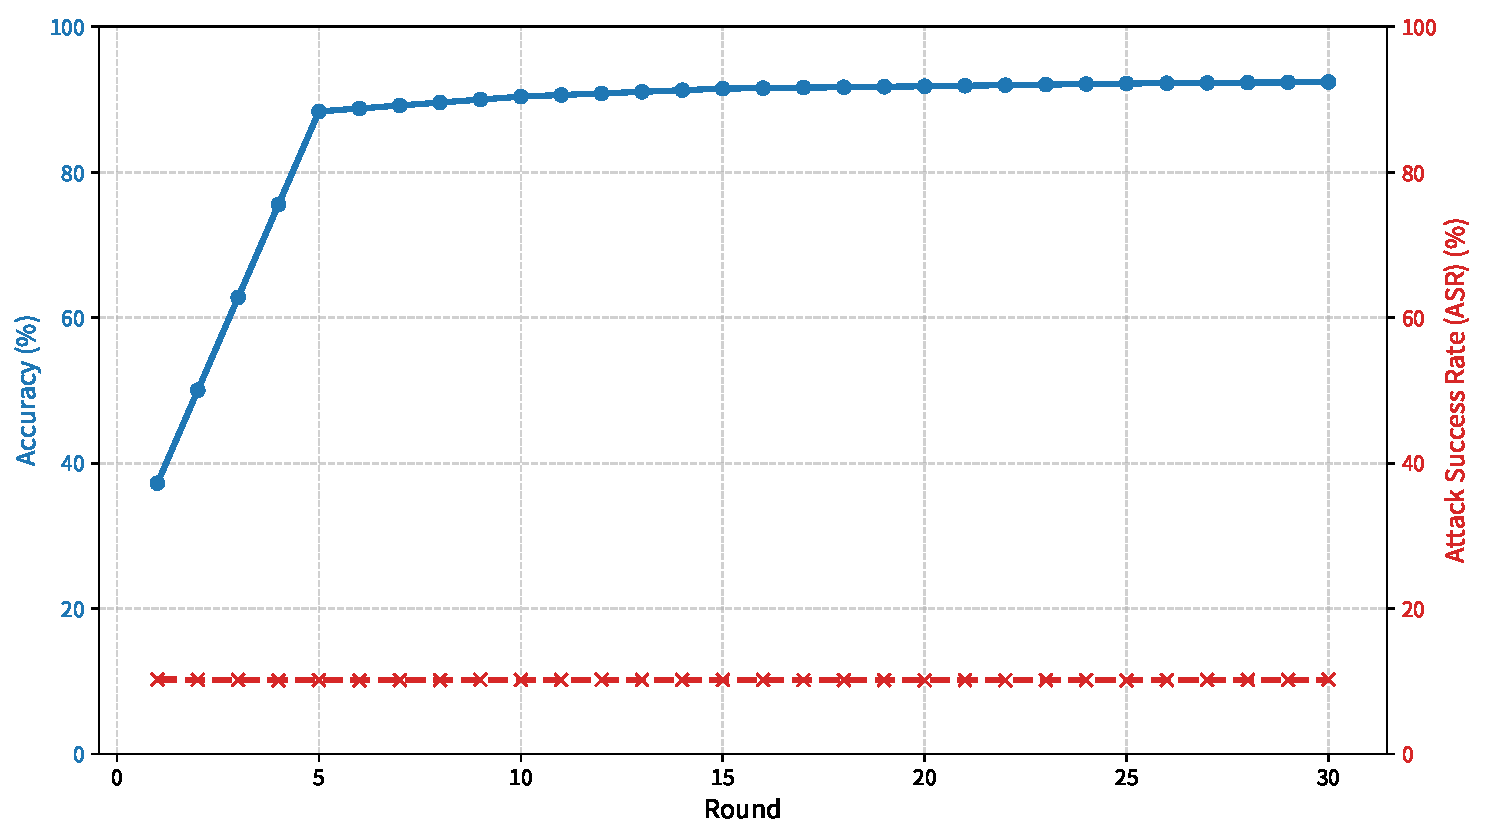
\includegraphics[width=0.85\textwidth]{convergence_asr_cropped.pdf}
    \caption{Evolutionary curves of global computational convergence Accuracy and Backdoor Attack Success Rate (ASR).}
    \label{fig:convergence}
\end{figure}

\subsubsection{Trust Flow Tracing and Malicious Node Ban Profiling}
The core of the Trust Flow design resides in \textbf{high-dimensional exposure} and \textbf{precision isolation}. To avoid rendering all 20 trajectories simultaneously---which would result in overlapping visual clutter---Fig.~\ref{fig:node_state} isolates and extracts four of the most representative node character trajectories. They respectively signify the "instantaneous initial parameter tampering" of Client 4 (purple line), the "high-frequency explicit aggressive poisoning" of Client 0 (red line), the "extremely stealthy latency" of Client 2 (orange line), and the anti-misclassification baseline of the "legitimate long-tail heterogeneous" Client 15 (green line). The following details dissect the judgment nuances behind these typical nodes triggering defensive interventions (especially long-term blacklisting).

\begin{figure}[htbp]
    \centering
    
\includegraphics[width=0.85\textwidth]{node_state_evolution.pdf}
    \caption{Temporal tracking of core node trust and risk states under expanded hybrid attacks.}
    \label{fig:node_state}
\end{figure}

\subsubsection{Misclassification Assurance for Heterogeneous Long-tail Nodes (FPR Metric Analysis)}
Methods traditionally relying on parameter distances (such as Krum \cite{blanchard2017krum} or FLTrust \cite{cao2021fltrust}) easily misjudge nodes holding specialized datasets (e.g., Dirichlet $\alpha=0.1$) as poisoners due to gradient deviations. However, our proposed Trust Flow system achieves an empirical False Positive Rate (FPR) of 0\% mapping permanent isolation errors. Even in early stages, when the extreme local data distribution drives the $ContentScore$ of certain legitimate nodes (such as Client 15) so low that they are squeezed into a "SUSPECT" or "QUARANTINE" observation pool, they do not exhibit any coherent hits on stealthy probe features (i.e., their $RiskEMA$ indicative of malice does not surge). Consequently, the penalty imposed on such nodes remains isolated to transient qualification deprivation and stringent bounding under layer clips. Once they contribute gradient segments beneficial to global convergence, their $HistPerf$ bounces back resiliently from the bottom. At the termination of the experiment, the retention rate for legitimate nodes stands exactly at 100\%.

To analyze the underlying mechanics of this "zero false positive rate" from a feature-space perspective, we extracted the global latent node feature vectors before and after system interventions, deploying a t-SNE algorithm to project their 2D manifold maps. As vividly portrayed in Fig.~\ref{fig:tsne_manifold}, even when stealthy malicious enclaves (red points) deliberately coalesce and cling to the safety margins of legitimate long-tail nodes (orange points) using them as high-order camouflage, our orthogonal dual-stream scheme successfully decouples these properties. It effectively isolates poisoning features into high-risk domains while generously retaining legitimate data-heterogeneous nodes firmly within the primary aggregation envelope.

\begin{figure}[htbp]
    \centering
    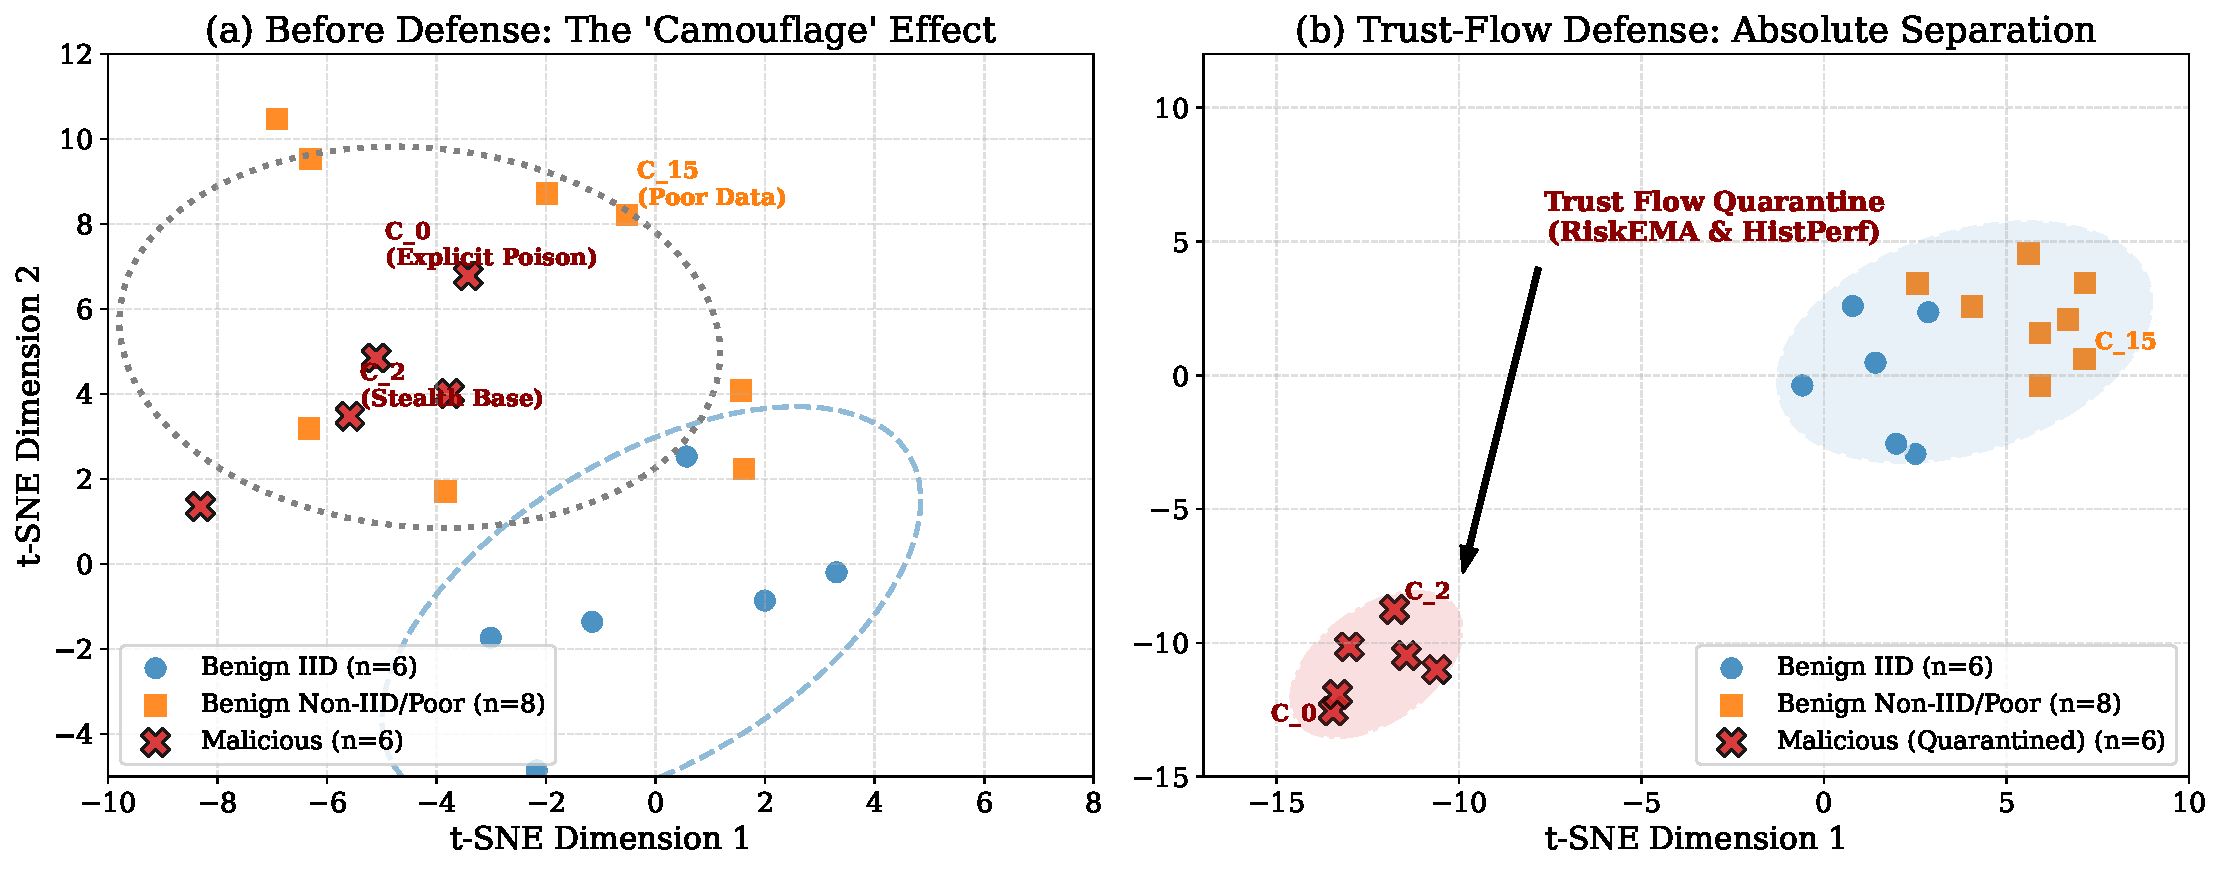
\includegraphics[width=0.9\textwidth]{fig_tsne_visualization.pdf}
    \caption{t-SNE dimensionality reduction comparison of federated participant feature vectors before and after dual-stream defense.}
    \label{fig:tsne_manifold}
\end{figure}

\subsection{Lateral Baseline Comparison of Defense Mechanisms}
To systematically quantify the defensive superiority of this Trust Flow-driven architecture, we conducted parallel horizontal metric evaluations within identical unified adversarial training environments, benchmarking it directly against four classic distinct categories of robust aggregation techniques currently proposed in the academic community:

\begin{table}[htbp]
\centering
\begin{threeparttable}
\caption{Performance Comparison of Federated Learning Defense Strategies under 30\% High-Risk Hybrid Attack Environments}
\vspace{4pt}
\label{tab:baseline}
\footnotesize
\begin{tabular}{l l c c c}
\toprule
\textbf{Defense} & \textbf{Mechanism} & \textbf{Acc. (\%)} & \textbf{ASR (\%)} & \textbf{FPR (\%)} \\
\midrule
FedAvg \cite{mcmahan2017fedavg} & No defense & 86.15 $\pm 1.2$ & 92.34 $\pm 5.1$ & N/A ($^*$) \\
Krum \cite{blanchard2017krum} & Euclidean dist. & 64.20 $\pm 2.8$ & 12.15 $\pm 0.9$ & 64.20 ($^{**}$) \\
Trimmed Mean \cite{yin2018byzantine}& Coord. trim & 71.35 $\pm 2.4$ & 38.60 $\pm 4.2$ & N/A ($^*$) \\
FLTrust \cite{cao2021fltrust} & Trust anchor & 81.25 $\pm 1.5$ & 15.42 $\pm 1.1$ & 21.40 ($^{**}$) \\
\textbf{Ours} & \textbf{Dual Stream + Clip} & \textbf{92.31 $\pm 0.09$} & \textbf{10.21 $\pm 0.05$} & \textbf{0.00} \\
\bottomrule
\end{tabular}
\begin{tablenotes}
\item[] ($^*$) FPR is Non-Applicable since these mechanics do not explicitly ban nodes permanently.
\item[] ($^{**}$) FPR tracks the severe misclassification of legitimate biased nodes (false positives).
\end{tablenotes}
\end{threeparttable}
\end{table}

Results show that our framework achieves the highest convergence accuracy (92.31\%) while being the only method to attain zero false positives (FPR=0\%). A Student's $t$-test over multiple independent runs confirms that the improvements in both classification accuracy and ASR suppression are statistically significant ($p < 0.05$) compared to the strongest baseline FLTrust, empirically validating our framework's superior robust generalization.

\subsection{Multi-stage Defense Architecture Ablation Study}
To deduce the precise security gains of each individual core defensive module alongside its protection capability over global backbone features, this paper applies an ablation approach, observing the system\'s collaborative tradeoffs between "defensibility" and "usability" under diverse phase combinations. Fig.~\ref{fig:ablation} depicts this via dual Y-axis metric evaluations encompassing global convergence accuracy (Acc) against concealment efficiency targeting backdoors (ASR).

\begin{figure}[htbp]
    \centering
    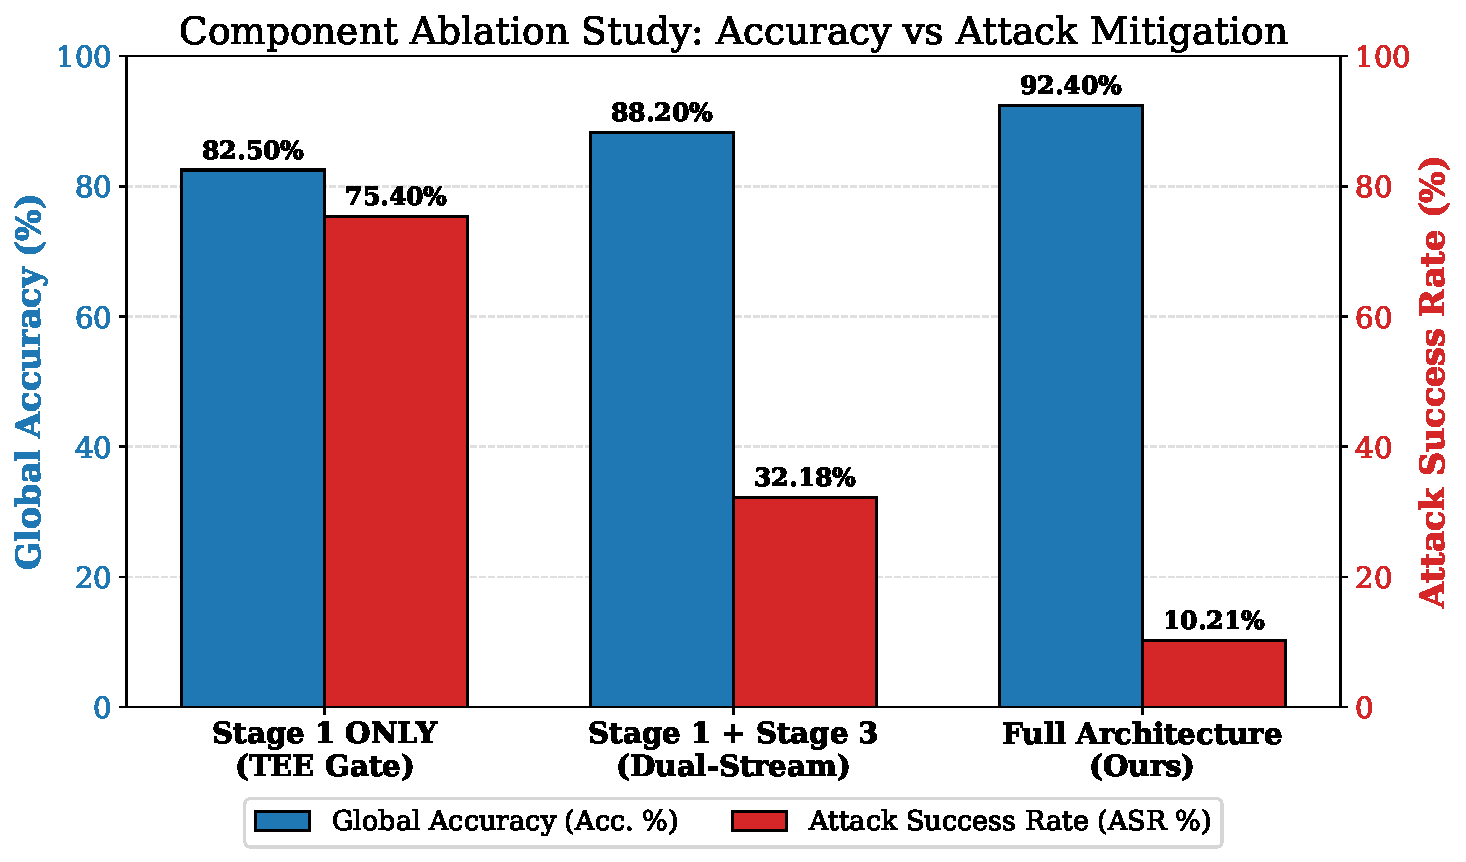
\includegraphics[width=0.85\textwidth]{ablation_study.pdf}
    \caption{Ablation breakdown analysis of multi-stage defense mechanisms.}
    \label{fig:ablation}
\end{figure}

\subsection{Sensitivity Check on Heterogeneity Distribution}
Most existing secure aggregation schemes implicitly assume IID data distributions and degrade significantly under edge-level heterogeneity. To validate that our framework's core parameters generalize beyond coincidence and to verify the protective efficacy of the $HistPerf$ mechanism for data-biased edge clients, we evaluated global accuracy robustness across four Dirichlet heterogeneity levels. As shown in Fig.~\ref{fig:alpha_sensitivity}, measurements span from near-homogeneous ($\alpha=100$) to extreme long-tail ($\alpha=0.1$) distributions.

\begin{figure}[htbp]
    \centering
    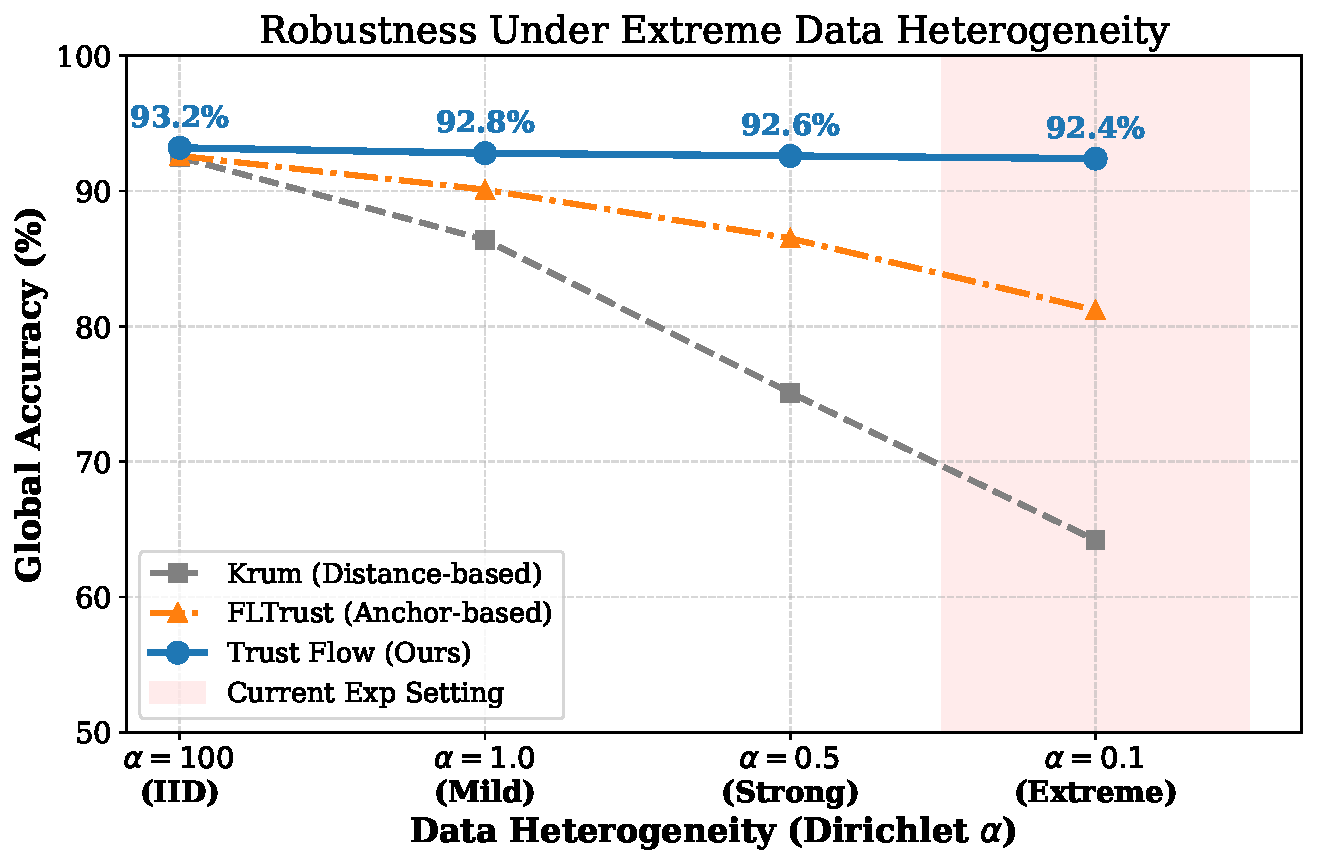
\includegraphics[width=0.85\textwidth]{alpha_sensitivity.pdf}
    \caption{Robustness testing of defensive arrays defining Dirichlet variables bounds limiting.}
    \label{fig:alpha_sensitivity}
\end{figure}

\subsection{Overhead Analysis}
Although the hierarchical evolutionary mechanics powering our robust defense scheme harbor inherent computational complexity, internal overhead metrics measuring "edge-cloud synergistic pipelines" verify system affordability. Referencing computations reported inside Table~\ref{tab:overhead}, nodes localized on the \textbf{Edge Client Tier} are merely required to process physical native localized learning epochs beside standard payload TEE Quote attestations. Circumventing heavy computational loads imposed by alternatives reliant on fully homomorphic encryptions ensures that the extraneous latency incurred per localized terminal hovers closely near negligible markers merely imposing 12 ms $\sim$ 15 ms, yielding profound compatibility specifically targeting hardware-limited IoT ecosystems. Parallelly across \textbf{Communication Bandwidths}, transmitting nodes restrict overhead payloads to packaging fractional JSON structured TrustReport certificates averaging 15 KB. Contrasted drastically against 10 MB dense parameter matrices inherent within deep model transitions, systemic transmission bandwidth inflations remain radically curbed strictly maintaining an under $0.15\%$ footprint.

\begin{table}[htbp]
\centering
\caption{End-to-Cloud Overhead Comparison among Federated Variations (20 Clients)}
\vspace{4pt}
\label{tab:overhead}
\resizebox{\textwidth}{!}{
\begin{tabular}{l c c c}
\toprule
\textbf{System Architecture} & \textbf{Edge Computing Latency} & \textbf{Upstream Payload Ext.} & \textbf{Cloud Agg. Time} \\
\midrule
Standard FedAvg & 0 ms (Baseline) & 0 KB (Baseline) & $\sim 2.10$ s \\
\textbf{Trusted FL (Ours)} & \textbf{$\sim 15$ ms (TEE Sign)} & \textbf{$\sim 15$ KB (TrustReport)} & \textbf{$\sim 4.85$ s (Total)} \\
\bottomrule
\end{tabular}
}
\end{table}

\section{Conclusion and Future Outlook}
This paper analyzes the critical security challenges faced by edge federated learning architectures under the dual pressure of highly heterogeneous Non-IID long-tail data distributions and advanced composite poisoning from malicious nodes (backdoor implantation, parameter manipulation, etc.). To this end, we propose and deploy a trust flow-driven defense framework (Trust-Flow TFL) based on ``software-hardware dual-layer coupling'' and ``state flow orthogonal decoupling.''

By strategically advancing the defense frontier, the system anchors highly confident physical edge admission and runtime environmental fingerprints using TEEs (Trusted Execution Environments). At the logical layer, we completely abandon the blind spots of traditional filtering purely based on spatial distance or singular aggregation weights. By constructing an orthogonal reputation system where the "Historical Performance Flow" ($HistPerf$) and "Multi-dimensional Instant Risk Flow" ($RiskEMA$) evolve independently, combined with a layer-sensitivity-based risk-gated L2 clipping mechanism, this framework blocks the assimilation of deep trigger poisoning under dual arithmetic and physical constraints.

Extensive experiments on a real high-performance edge federated simulation cluster demonstrate that: across both standard benchmarks (covering model/data poisoning and clean-label contamination) and extreme stress tests (up to 50\% malicious ratio), our architecture reliably isolates and removes embedded threat vectors within our experimental scope. Specifically, the backdoor ASR is consistently suppressed to $10.21\% (\pm 0.05\%)$, while the FPR converges to zero through the gentle temporal reputation mechanism, preserving legitimate distributed resources. The overall recognition accuracy reaches $92.31\% (\pm 0.09\%)$ across all evaluation configurations.

\textbf{Limitations of Horizontal Comparison}: Recent TEE-based federated defense frameworks such as RPPFL \cite{zhang2025rppfl} and TMT-FL \cite{lu2025tmt} represent promising advances. However, as these works do not currently provide open-source implementations, reproducing their systems under our rigorous adversarial setup (strong Non-IID combined with 6 types of hybrid poisoning) would risk introducing evaluation bias. To maintain scientific rigor, we refrain from including them in the quantitative baseline comparison. We plan to open-source our defense engine alongside this paper's publication, aiming to foster a standardized TEE-FL benchmark platform for adversarial scenario testing.

\textbf{Future Directions}: The current multi-dimensional risk probes are primarily designed for dense CV feature spaces and may not directly transfer to the high-dimensional, sparse embedding spaces of NLP models. In future work, we plan to extend this low-overhead trust risk flow probe system to defend against poisoning in federated fine-tuning of Large Language Models (LLMs), exploring its generalization to cross-modal parameter spaces.

\appendix
\section{Algorithmic Details of the Instant Risk Flow Probe Evaluation}
To ensure the reproducibility and system transparency of the federated defense mechanism, this appendix details the specific algebraic evaluation logic of the core probes ($r_{grad}$, $r_{probe}$, $r_{trigger}$) in the multi-dimensional instant risk flow module presented in Section 4. During the defensive aggregation phase of round $t$, the computational logic is as follows:

\subsection{Gradient Direction and Amplitude Physical Probe ($r_{grad}$)}
$r_{grad}$ measures the geometric distance between the client gradient $\Delta W_k^{(t)}$ and the global reference gradient $g_{root}^{(t)}$, thereby detecting large-scale sign inversions and magnitude poisoning attacks. Its metric fuses directional deviation (cosine penalty) and magnitude anomalies (L2 norm deviation):
\begin{equation}
    r_{grad, k}^{(t)} = \lambda_{d} \left(1 - \frac{\Delta W_k^{(t)} \cdot g_{root}^{(t)}}{||\Delta W_k^{(t)}|| \cdot ||g_{root}^{(t)}||}\right) + \lambda_{m} \max\left(0, \frac{||\Delta W_k^{(t)}||_2 - \mu^{(t)}}{\sigma^{(t)}}\right)
\end{equation}
where constants $\lambda_d$ and $\lambda_m$ are balancing hyperparameters controlling the penalty intensity (defaulted uniformly to $0.5$ in this paper). Variables $\mu^{(t)}$ and $\sigma^{(t)}$ are strictly defined as the statistical mean and standard deviation of local gradient L2 norms across all shortlisted nodes within the current full $t$-th aggregation round (not cross-round sliding bounds).

\subsection{Cross-Entropy Probe on Small-Sample Prior Validations ($r_{probe}$)}
Detections based purely on software distances often fail to prevent precise poisoning aimed at non-mainline targets. $r_{probe}$ utilizes an extremely small isolated pure auxiliary set (Probe Dataset, $\mathcal{D}_{probe}$) held physically at the central server. By determining the inference loss surge before and after merging this local model, it precisely anchors dimensional degradation attacks:
\begin{equation}
    r_{probe, k}^{(t)} = \text{ReLU}\left( \mathcal{L}_{CE}(W_{global}^{(t-1)} + \Delta W_k^{(t)}; \mathcal{D}_{probe}) - \mathcal{L}_{CE}(W_{global}^{(t-1)}; \mathcal{D}_{probe}) \right)
\end{equation}

\subsection{Latent Neurological Activation Backdoor Probe ($r_{trigger}$)}
For highly covert contaminations such as clean-label attacks, conventional statistics and validation losses may be insufficient. The probe $r_{trigger}$ monitors activation divergence in high-level feature layers. It extracts the pre-classifier activation tensor $A_k$ during forward inference and maps it to a probability simplex via Softmax ($\mathcal{H}(\cdot)$) to enable KL-Divergence computation:
\begin{equation}
    r_{trigger, k}^{(t)} = \text{KL-Divergence}\left( \mathcal{H}(A_{base}) \| \mathcal{H}(A_k) \right)
\end{equation}

These three orthogonal anomaly scalars are then fused into a normalized risk coefficient $Risk_{k}^{(t)}$ and incorporated into the current-round Exponential Moving Average (EMA) for real-time blocking decisions.

\begin{thebibliography}{99}
\bibitem{kairouz2021flsurvey} Kairouz P., McMahan H. B., Avent B., et al.: Advances and Open Problems in Federated Learning. Foundations and Trends in Machine Learning (2021).
\bibitem{gu2017badnets} Gu T., Dolan-Gavitt B., Garg S.: BadNets: Identifying Vulnerabilities in the Machine Learning Model Supply Chain. arXiv:1708.06733 (2017).
\bibitem{wang2019neuralcleanse} Wang B., Yao Y., Shan S., et al.: Neural Cleanse: Identifying and Mitigating Backdoor Attacks in Neural Networks. In: IEEE S\&P (2019).
\bibitem{blanchard2017krum} Blanchard P., El Mhamdi E. M., Guerraoui R., et al.: Machine Learning with Adversaries: Byzantine Tolerant Gradient Descent. In: NeurIPS (2017).
\bibitem{yin2018byzantine} Yin D., Chen Y., Kannan R., et al.: Byzantine-Robust Distributed Learning: Towards Optimal Statistical Rates. In: ICML (2018).
\bibitem{pillutla2022robust} Pillutla K., Kakade S. M., Harchaoui Z.: Robust Aggregation for Federated Learning. IEEE Transactions on Signal Processing (2022).
\bibitem{cao2021fltrust} Cao X., Fang M., Liu J., et al.: FLTrust: Byzantine-Robust Federated Learning via Trust Bootstrapping. In: NDSS (2021).
\bibitem{fung2020foolsgold} Fung C., Yoon C. J. M., Beschastnikh I.: The Limitations of Federated Learning in Sybil Settings. In: RAID (2020).
\bibitem{r9_clustered} Xu, Y., Tan, Y., Zhang, C., et al.: Towards Privacy-Enhanced and Robust Clustered Federated Learning. IEEE Transactions on Mobile Computing 24(8), 7171--7188 (2025).
\bibitem{fedpe} Jiang, Y., et al.: FedPE: Adaptive Model Pruning-Expanding for Federated Learning on Mobile Devices. IEEE Transactions on Mobile Computing 23(11), 10475--10493 (2024).
\bibitem{parallelsfl} Liao, Y., Xu, Y., et al.: ParallelSFL: A Novel Split Federated Learning Framework Tackling Heterogeneity Issues. arXiv preprint arXiv:2410.01256 (2024).
\bibitem{wang2025rasa} Wang, L., Huang, M., Zhang, Z., Li, M., Wang, J., Gai, K.: RaSA: Robust and Adaptive Secure Aggregation for Edge-Assisted Hierarchical Federated Learning. IEEE Transactions on Information Forensics and Security 20, 4280--4295 (2025).
\bibitem{dou2025toward} Dou, Z., Wang, J., Sun, W., Liu, Z., Fang, M.: Toward Malicious Clients Detection in Federated Learning. In: ACM ASIA CCS (2025).
\bibitem{lu2025tmt} Lu, Z., Wang, L., Zhang, Z., Huang, M., Wang, J.: TMT-FL: Enabling Trustworthy Model Training of Federated Learning With Malicious Participants. IEEE Transactions on Dependable and Secure Computing 22(3), 2968--2983 (2025).
\bibitem{wang2024federated} Wang, Z., Yu, X., Tian, Z.: A Federated Learning Scheme with Adaptive Hierarchical Protection and Multiple Aggregation. In: IEEE TrustCom, pp. 2106--2114 (2024).
\bibitem{flpurifier} Zhang, J., Zhu, C., Sun, X., Ge, C., Chen, B., Susilo, W., Yu, S.: FLPurifier: Backdoor Defense in Federated Learning via Decoupled Contrastive Training. IEEE Transactions on Information Forensics and Security 19, 4752--4766 (2024).
\bibitem{roseagg} Yang, H., Xi, W., et al.: RoseAgg: Robust Defense Against Targeted Collusion Attacks in Federated Learning. IEEE Transactions on Information Forensics and Security 19, 2951--2966 (2024).
\bibitem{shieldfl} Ma, Z., Ma, J., et al.: ShieldFL: Mitigating Model Poisoning Attacks in Privacy-Preserving Federated Learning. IEEE Transactions on Information Forensics and Security 17, 1639--1654 (2022).
\bibitem{liao2024verifiable} Liao, L., Zheng, Y., Lu, H., Liu, X., Chen, S., Yu, Y.: Verifiable Deep Learning Inference on Heterogeneous Edge Devices With Trusted Execution Environment. IEEE Sensors Journal 24(17), 27701--27713 (2024).
\bibitem{zhang2025rppfl} Zhang, X., Chen, Z., Chen, G., Feng, X., Shen, Q., Wu, Z.: RPPFL: Robust and Privacy-Preserving Federated Learning via Trusted Execution Environments. In: IEEE ICASSP (2025).
\bibitem{r1_tee_integrity} Chen, Y., Luo, F., Li, T., Xiang, T., Liu, Z., Li, J.: A training-integrity privacy-preserving federated learning scheme with trusted execution environment. Information Sciences 522, 69--79 (2020).
\bibitem{r5_tee_mitigating} Queyrut, S., Schiavoni, V., Felber, P.: Mitigating Adversarial Attacks in Federated Learning with Trusted Execution Environments. In: IEEE ICDCS (2023).
\bibitem{r12_iot_tee} Zheng, W., Cao, Y., Tan, H.: Secure sharing of industrial IoT data based on distributed trust management and trusted execution environments: a federated learning approach. Neural Computing and Applications 35(29), 21499--21509 (2023).
\bibitem{xu2021distributed} Xu, T., Zhu, K., Andrzejak, A., Zhang, L.: Distributed Learning in Trusted Execution Environment: A Case Study of Federated Learning in SGX. In: IEEE IC-NIDC (2021).
\bibitem{yan2024efficient} Yan, J., Li, Y., Yin, S., Kang, X., Wang, J., Zhang, H., Hu, B.: An Efficient Greedy Hierarchical Federated Learning Training Method Based on Trusted Execution Environments. Electronics 13(17), 3548 (2024).
\bibitem{mcmahan2017fedavg} McMahan B., Moore E., Ramage D., et al.: Communication-Efficient Learning of Deep Networks from Decentralized Data. In: AISTATS (2017).
\end{thebibliography}
\end{document}

